\clearpage
\section{Raw results from the first U.S. complementary survey}\label{app:raw_results_US1}

\begin{figure}[h!]
    \caption{Correct answers to comprehension questions. (Questions \ref{q:understood_gcs}-\ref{q:understood_both})}\label{fig:understood_each}
    \makebox[\textwidth][c]{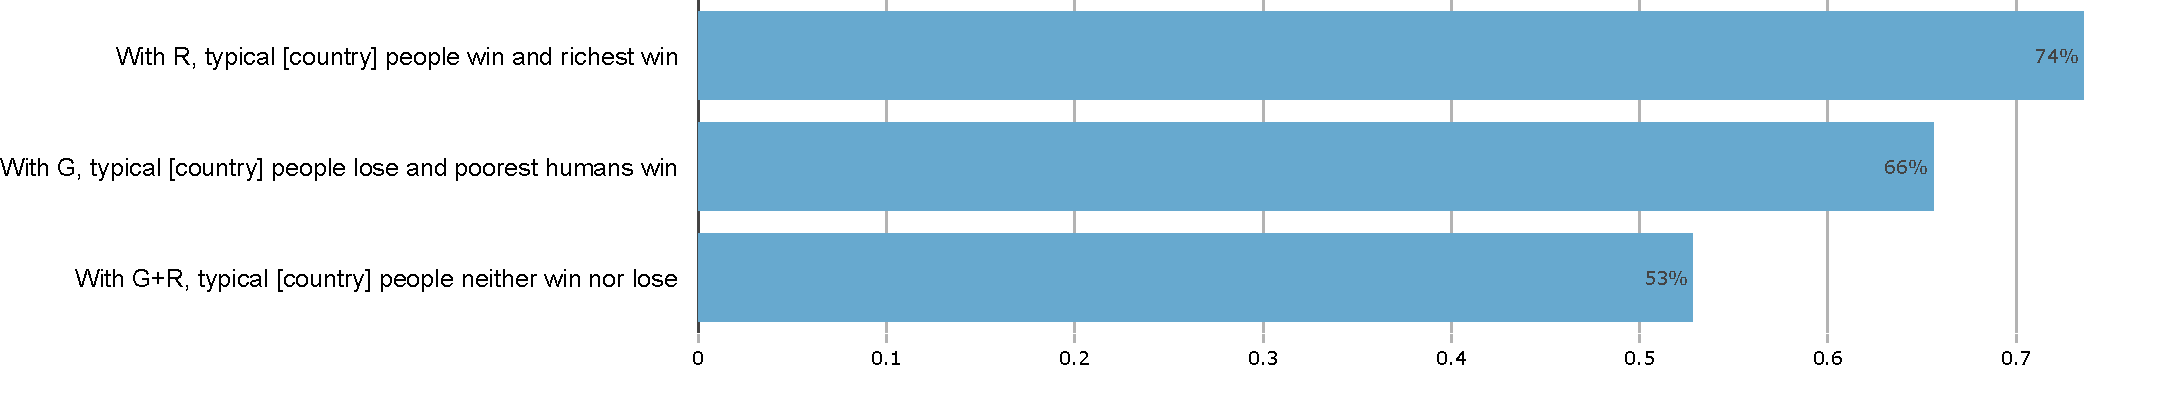
\includegraphics[width=\textwidth]{../figures/US1/understood_each.pdf}} 
\end{figure}

\begin{figure}[h!]
    \caption{Number of correct answers to comprehension questions. (Questions \ref{q:understood_gcs}-\ref{q:understood_both})}\label{fig:understood_score}
    \makebox[\textwidth][c]{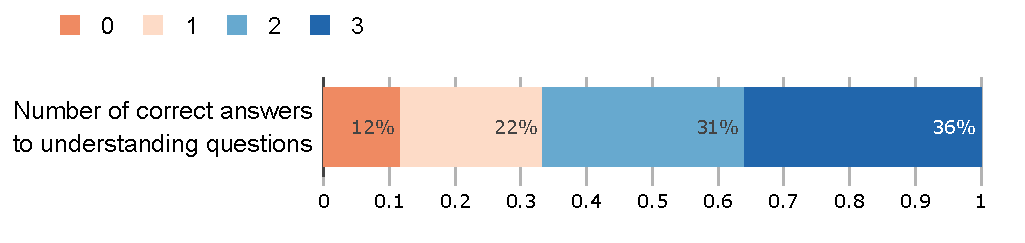
\includegraphics[width=.8\textwidth]{../figures/US1/understood_score.pdf}} 
\end{figure}

\begin{figure}[h!]
    \caption{Support for the GCS, NC and the combination of GCS, NR and C. (Questions \ref{q:gcs_support}, \ref{q:nr_support} and \ref{q:crg_support})}\label{fig:support_binary}
    \makebox[\textwidth][c]{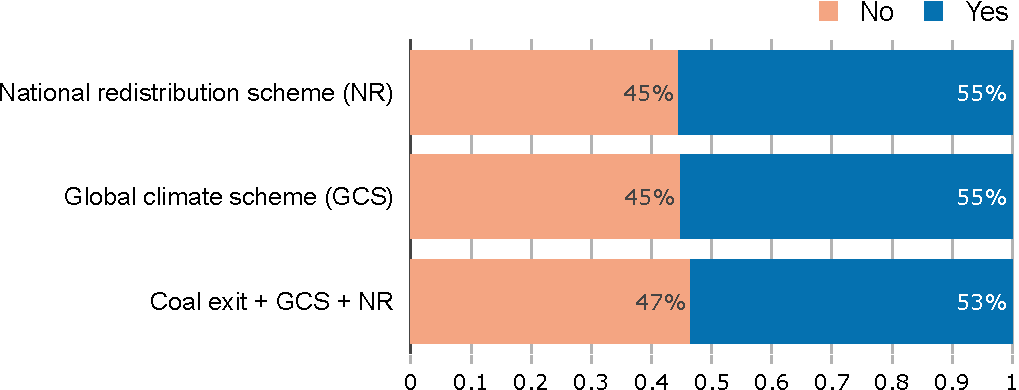
\includegraphics[width=.9\textwidth]{../figures/US1/support_binary.pdf}} 
\end{figure}

\begin{figure}[h!]
    \caption{Beliefs regarding the support for the GCS and NR. (Questions \ref{q:gcs_belief} and \ref{q:nr_belief})}\label{fig:belief}
    \makebox[\textwidth][c]{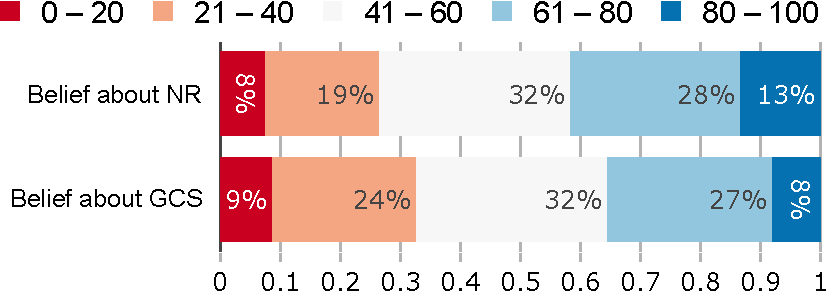
\includegraphics[width=.8\textwidth]{../figures/US1/belief.pdf}} 
\end{figure}

\begin{figure}[h!]
    \caption{List experiment. (Question \ref{q:list_exp})}\label{fig:list_exp}
    \makebox[\textwidth][c]{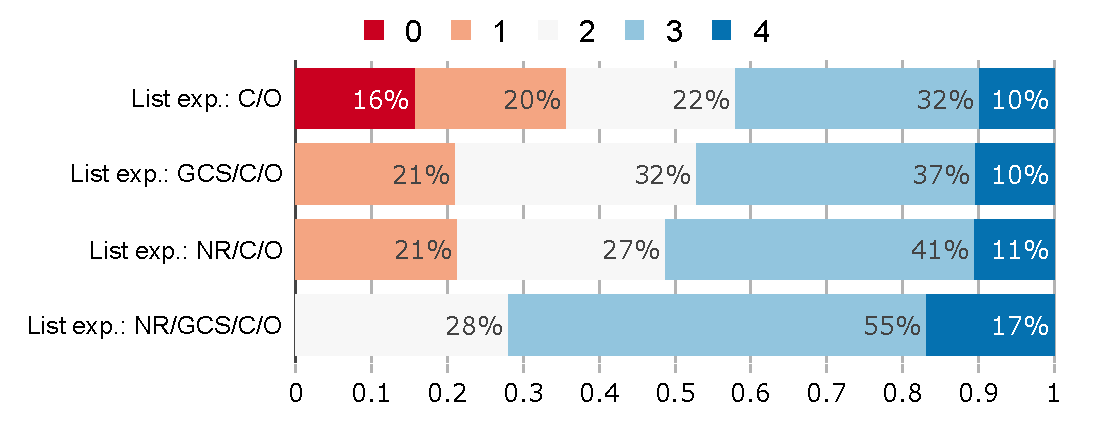
\includegraphics[width=\textwidth]{../figures/US1/list_exp.pdf}} 
\end{figure}

\begin{figure}[h!]
    \caption{Conjoint analyses. (Questions \ref{q:conjoint_a}-\ref{q:conjoint_d})}\label{fig:conjoint}
    \makebox[\textwidth][c]{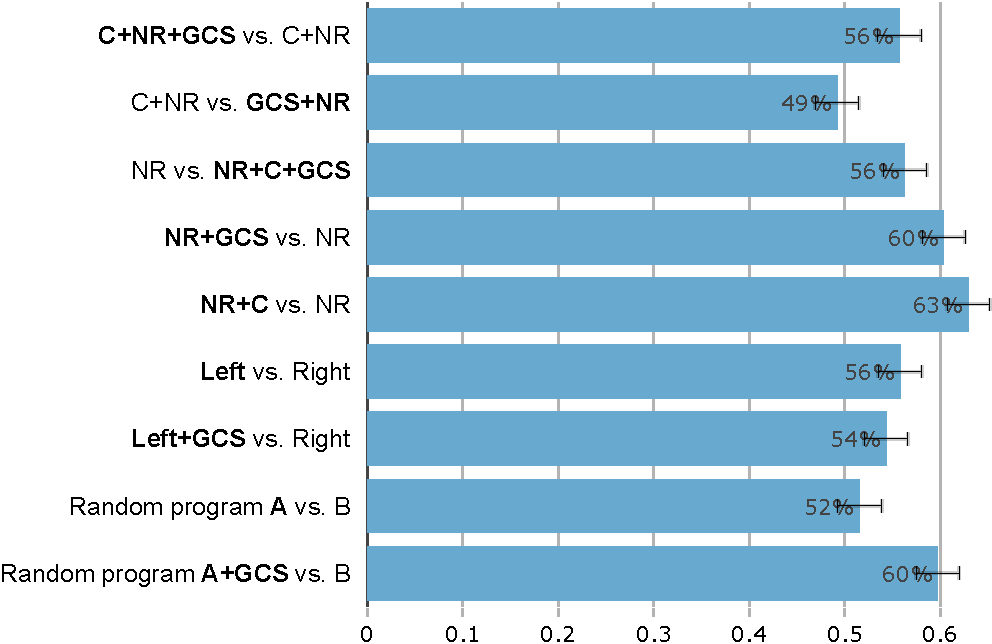
\includegraphics[width=\textwidth]{../figures/US1/conjoint.pdf}} 
\end{figure}

\begin{figure}[h!] % already in text
    \caption{[Asked only to non-Republicans] Conjoint analysis n°4: random programs at the Democratic primary. (Question \ref{q:conjoint_r})}\label{fig:ca_r}
    \makebox[\textwidth][c]{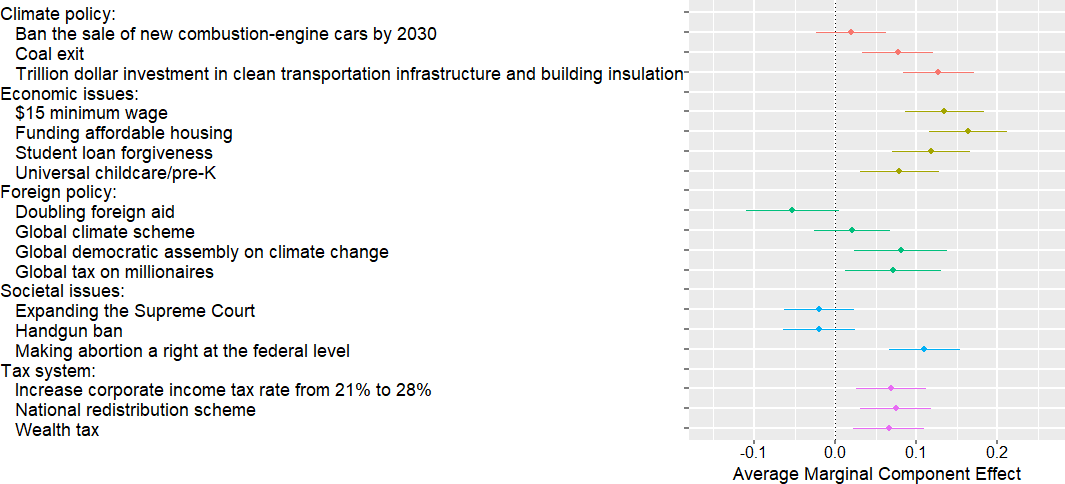
\includegraphics[width=\textwidth]{../figures/US1/ca_r.png}} 
\end{figure}

\begin{figure}[h!]
    \caption{Donation in case of lottery win. (Question \ref{q:donation})}\label{fig:donation}
    \makebox[\textwidth][c]{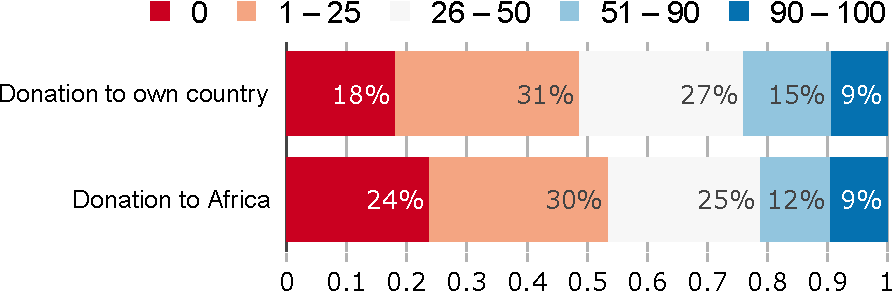
\includegraphics[width=.8\textwidth]{../figures/US1/variables_donation.pdf}} 
\end{figure}

\begin{figure}[h!]
    \caption{Willingness to sign real-stake petition for the GCS or NR. (Question \ref{q:petition})}\label{fig:petition}
    \makebox[\textwidth][c]{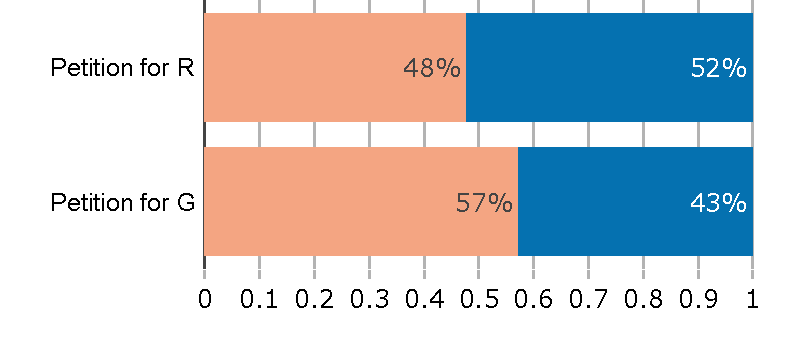
\includegraphics[width=.7\textwidth]{../figures/US1/variables_petition.pdf}} 
\end{figure}

\begin{figure}[h!] % already in text
    \caption{Support for various global policies. (Questions \ref{q:climate_policies} and \ref{q:other_policies})}\label{fig:support_likert}
    \makebox[\textwidth][c]{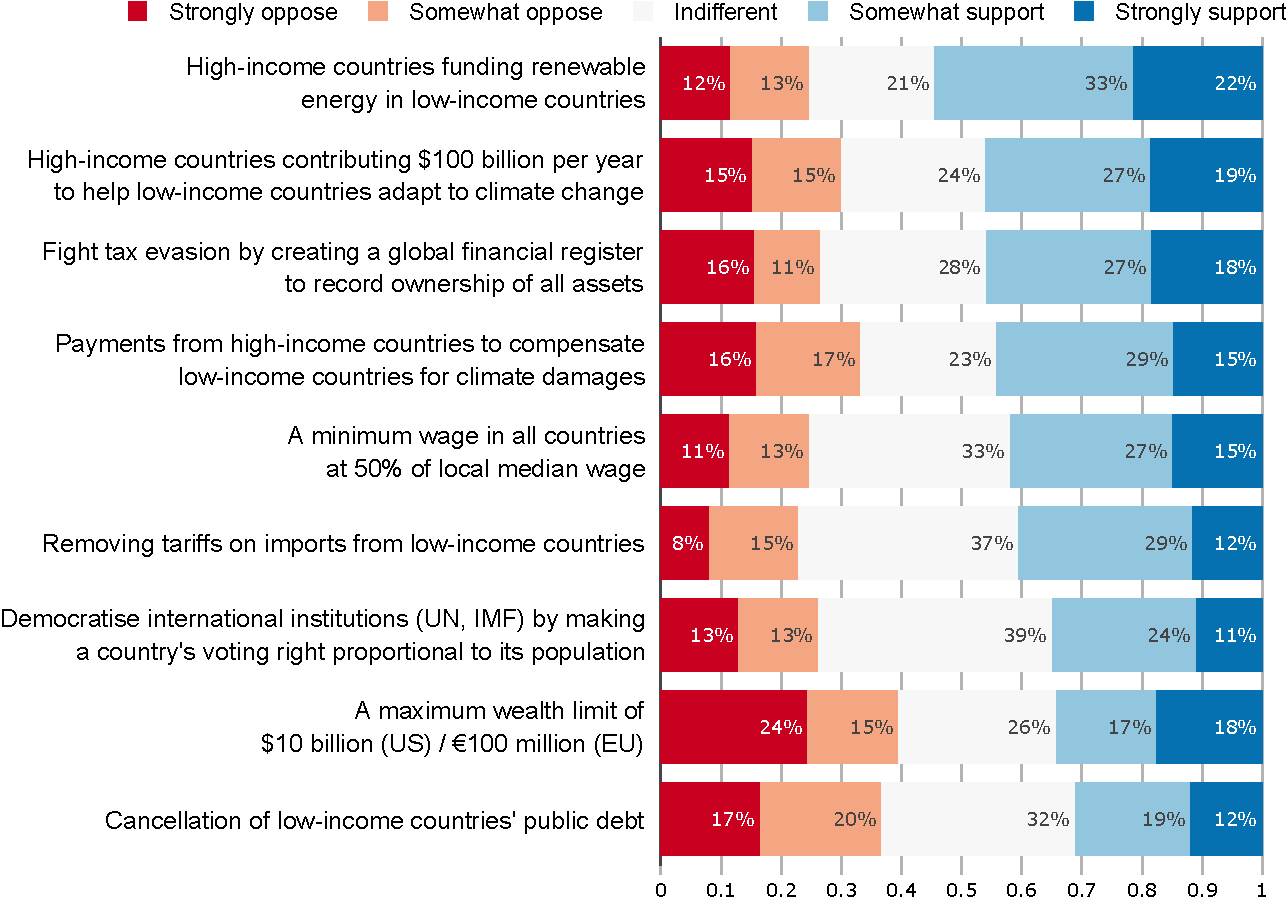
\includegraphics[width=\textwidth]{../figures/US1/support_likert.pdf}} 
\end{figure}

% \begin{figure}[h!]
%     \caption{label}\label{fig:climate_policies}
%     \makebox[\textwidth][c]{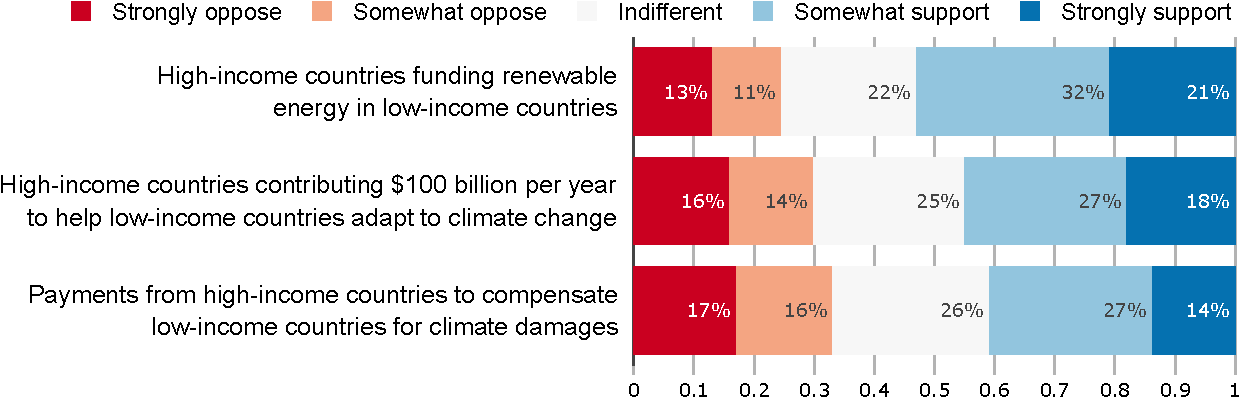
\includegraphics[width=\textwidth]{../figures/US1/climate_policies.pdf}} 
% \end{figure}

% \begin{figure}[h!]
%     \caption{label}\label{fig:global_policies}
%     \makebox[\textwidth][c]{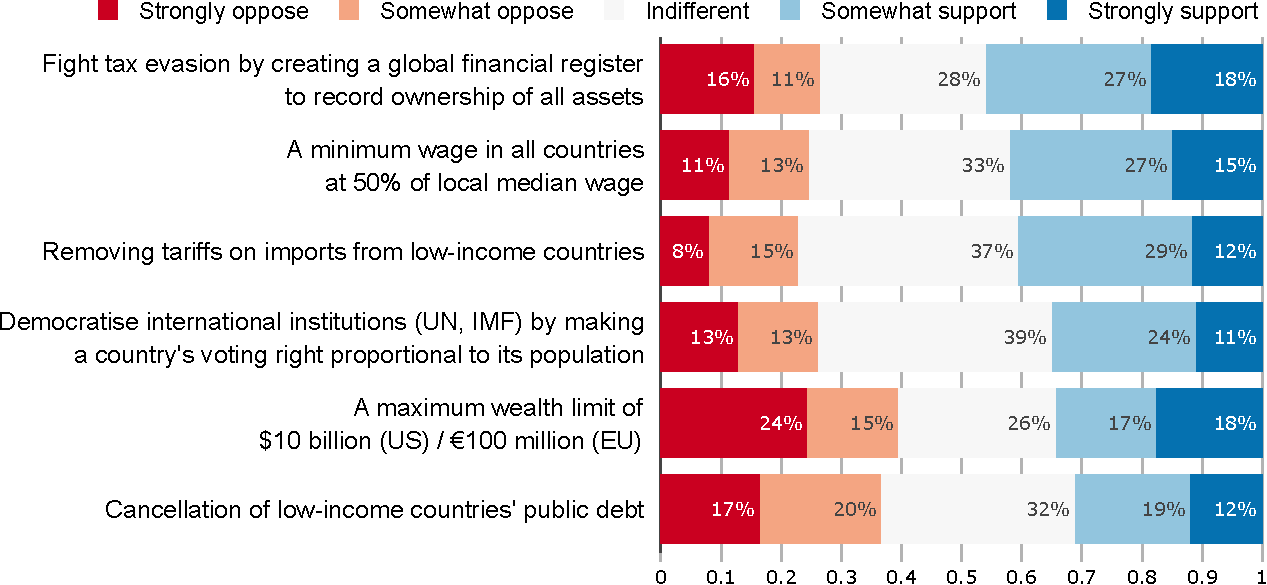
\includegraphics[width=\textwidth]{../figures/US1/global_policies.pdf}} 
% \end{figure}

\begin{figure}[h!]
    \caption{Attitudes regarding the evolution of U.S. foreign aid. (Question \ref{q:foreign_aid_raise_support})}\label{fig:foreign_aid_raise_support}
    \makebox[\textwidth][c]{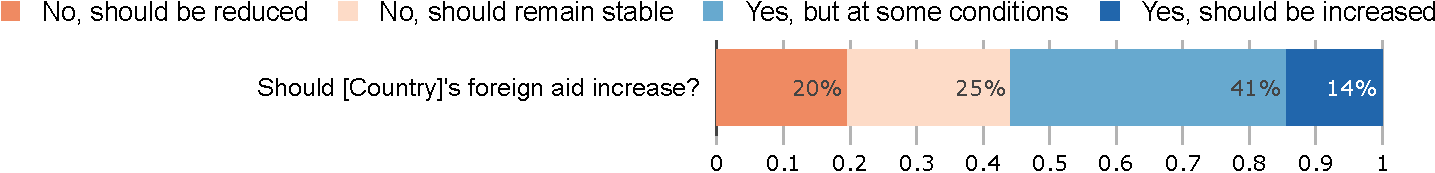
\includegraphics[width=\textwidth]{../figures/US1/foreign_aid_raise_support.pdf}} 
\end{figure}

\begin{figure}[h!]
    \caption{[Asked to those who wish an increase of foreign aid at some conditions.] Conditions at which foreign aid should be increased. (Question \ref{q:foreign_aid_condition})}\label{fig:foreign_aid_condition}
    \makebox[\textwidth][c]{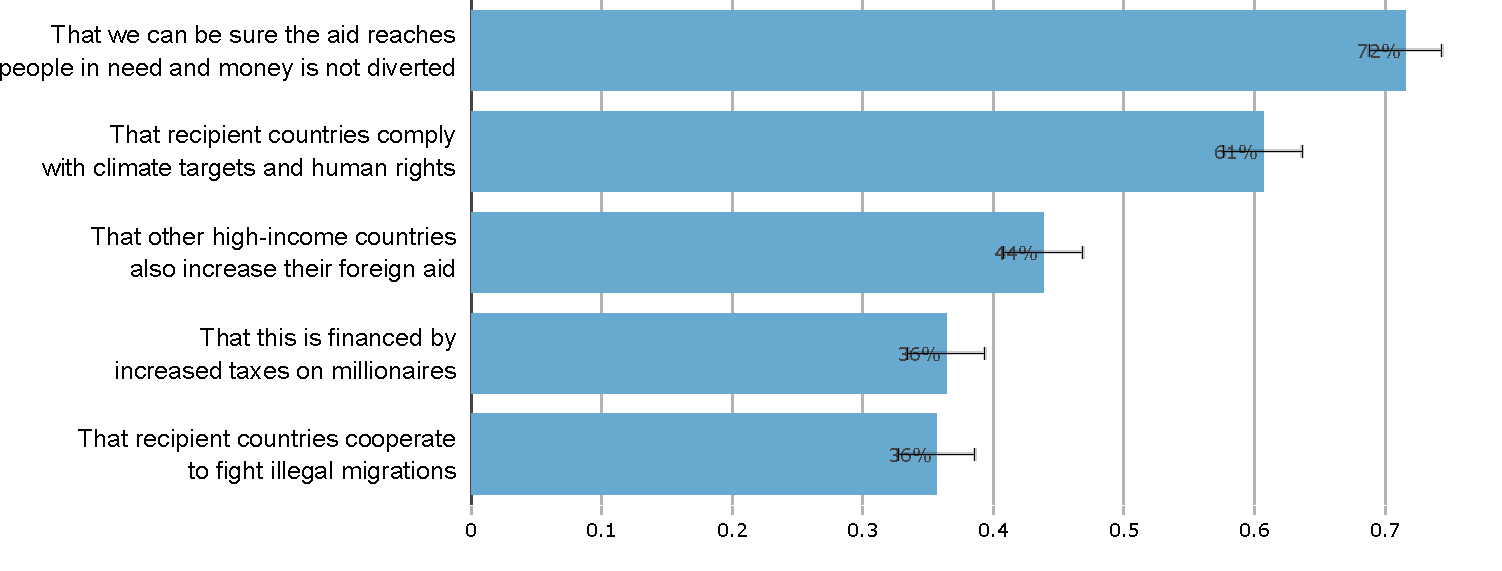
\includegraphics[width=\textwidth]{../figures/US1/foreign_aid_condition.pdf}} 
\end{figure}

\begin{figure}[h!]
    \caption{[Asked to those who wish a decrease or stability of foreign aid.] Reasons why foreign aid should not be increased. (Question \ref{q:foreign_aid_no})}\label{fig:foreign_aid_no}
    \makebox[\textwidth][c]{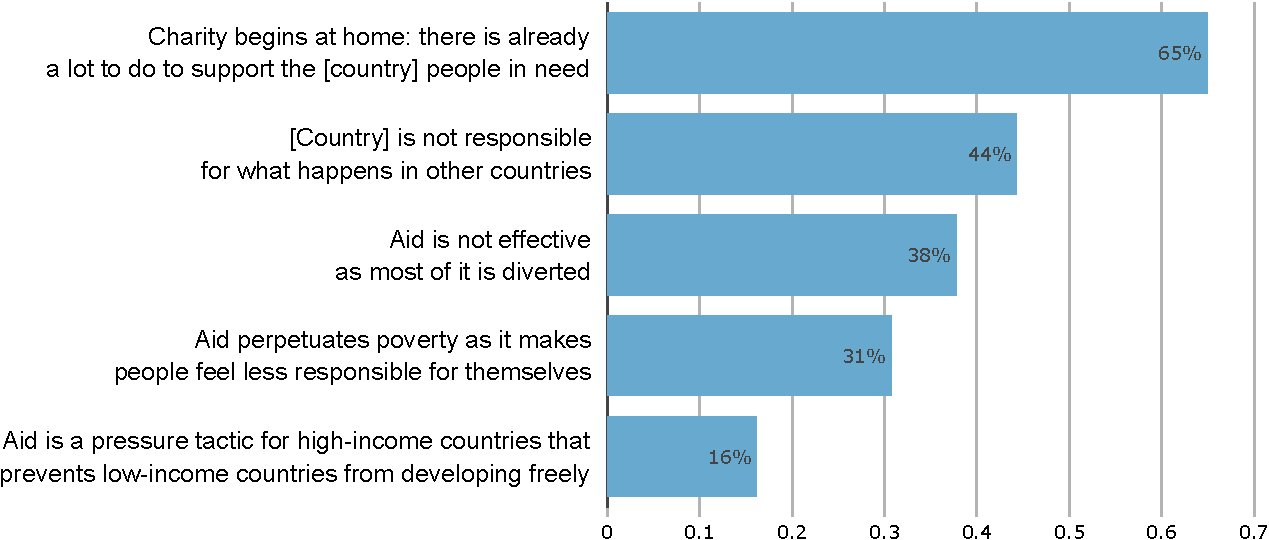
\includegraphics[width=\textwidth]{../figures/US1/foreign_aid_no.pdf}} 
\end{figure}

\begin{figure}[h!]
    \caption{Preferred approach of U.S. diplomats at international climate negotiations. (Question \ref{q:negotiation})}\label{fig:negotiation}
    \makebox[\textwidth][c]{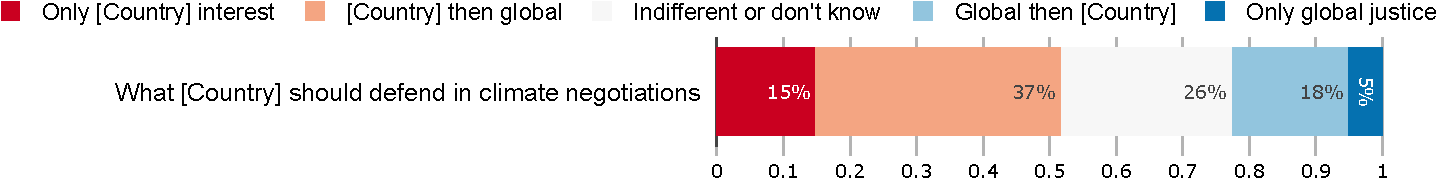
\includegraphics[width=\textwidth]{../figures/US1/negotiation.pdf}} 
\end{figure}

% \begin{figure}[h!]
%     \caption{label}\label{fig:vote}
%     \makebox[\textwidth][c]{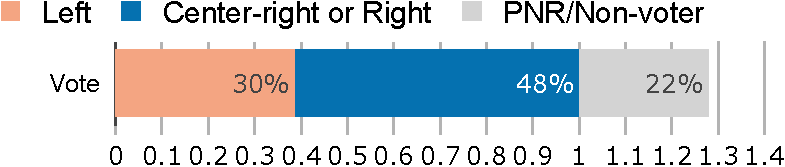
\includegraphics[width=\textwidth]{../figures/US1/vote.pdf}} 
% \end{figure}

\begin{figure}[h!]
    \caption{Extent to which selected issues are viewed as important problems. (Question \ref{q:problem})}\label{fig:problem}
    \makebox[\textwidth][c]{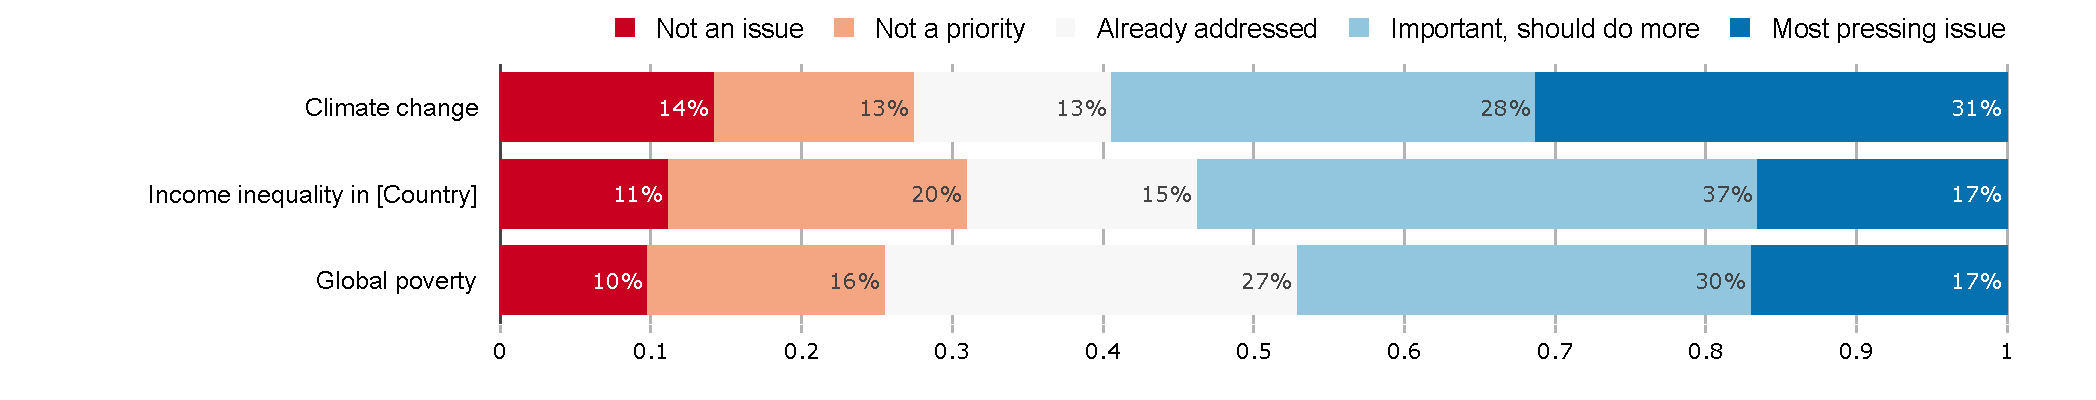
\includegraphics[width=\textwidth]{../figures/US1/problem.pdf}} 
\end{figure}

\begin{figure}[h!]
    \caption{Group defended when voting. (Question \ref{q:group_defended_agg})}\label{fig:group_defended_agg}
    \makebox[\textwidth][c]{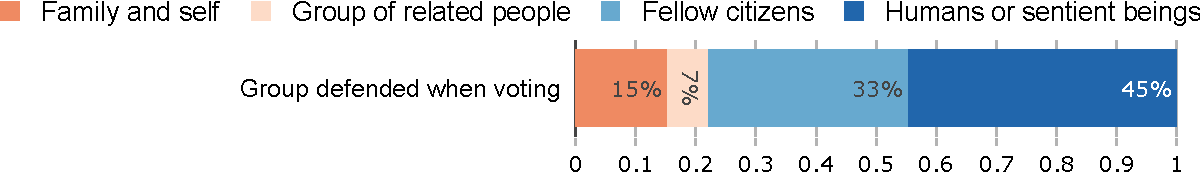
\includegraphics[width=\textwidth]{../figures/US1/group_defended_agg.pdf}} 
\end{figure}

% \begin{figure}[h!]
%     \caption{label}\label{fig:group_defended}
%     \makebox[\textwidth][c]{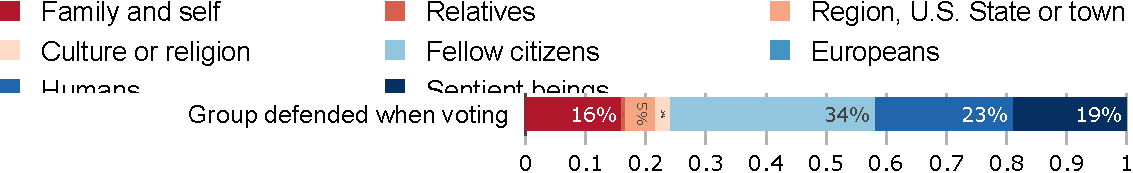
\includegraphics[width=\textwidth]{../figures/US1/group_defended.pdf}} 
% \end{figure}

\begin{figure}[h!] % already in text
    \caption{Prioritization of policies. (Question \ref{q:points_us})}\label{fig:points_us}
    \makebox[\textwidth][c]{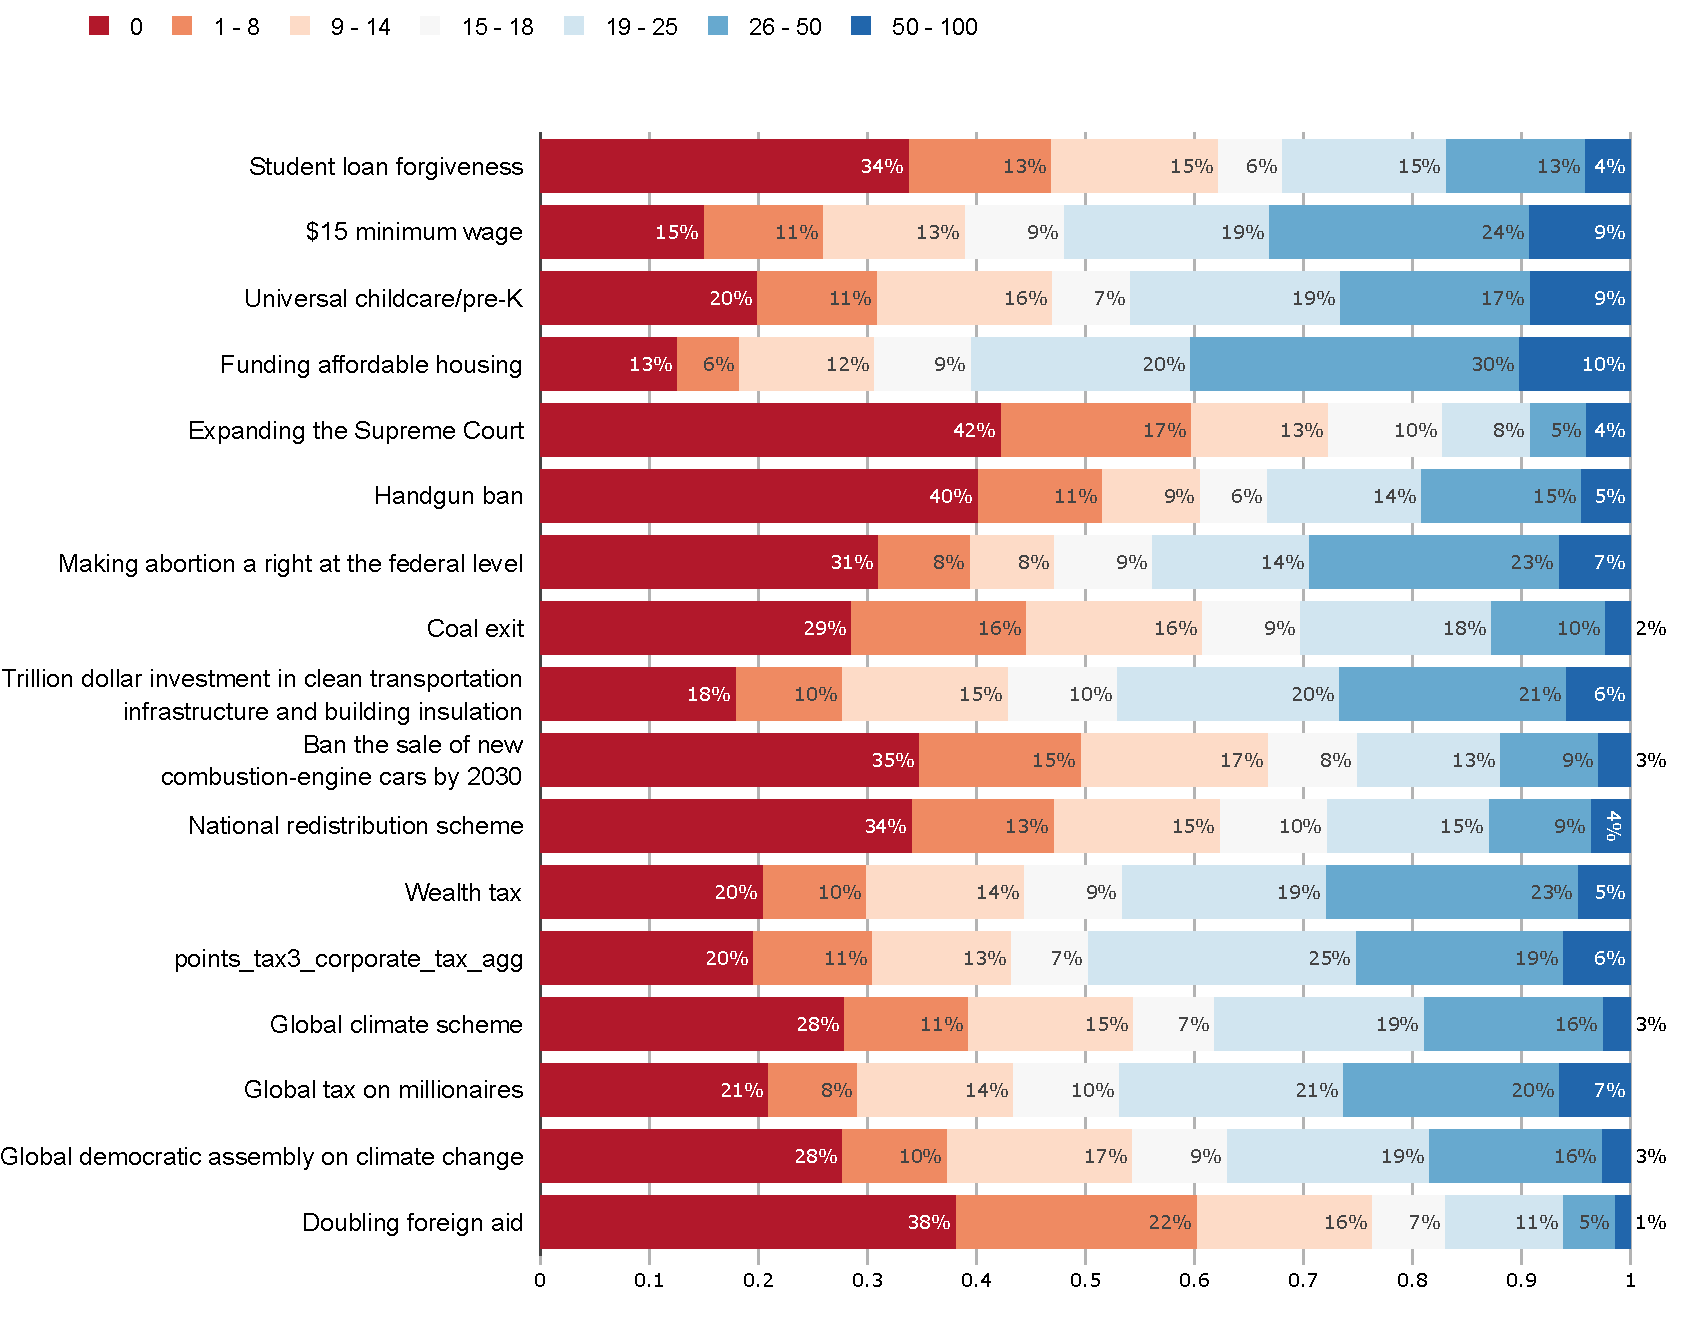
\includegraphics[width=\textwidth]{../figures/US1/points_us.pdf}} 
\end{figure}

% \begin{figure}[h!]
%     \caption{label}\label{fig:share_policies_supported}
%     \makebox[\textwidth][c]{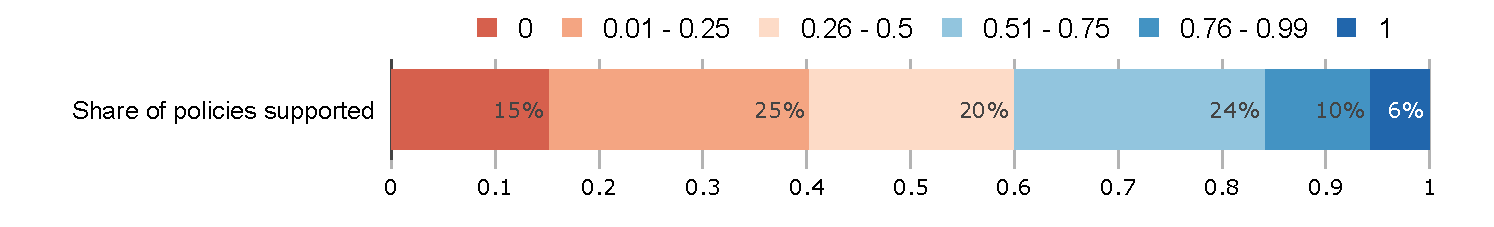
\includegraphics[width=\textwidth]{../figures/US1/share_policies_supported.pdf}} 
% \end{figure} % TODO? uncomment?

% \begin{figure}[h!]
%     \caption{label}\label{fig:vars}
%     \makebox[\textwidth][c]{\includegraphics[width=\textwidth]{../figures/US1/vars.pdf}} 
% \end{figure}

\clearpage
\section{Questionnaire of US1 %the first U.S. complementary 
survey}\label{app:questionnaire_US1}

\begin{figure}[h!]
    \caption{US1 survey structure}\label{fig:flow_US1}
    \makebox[\textwidth][c]{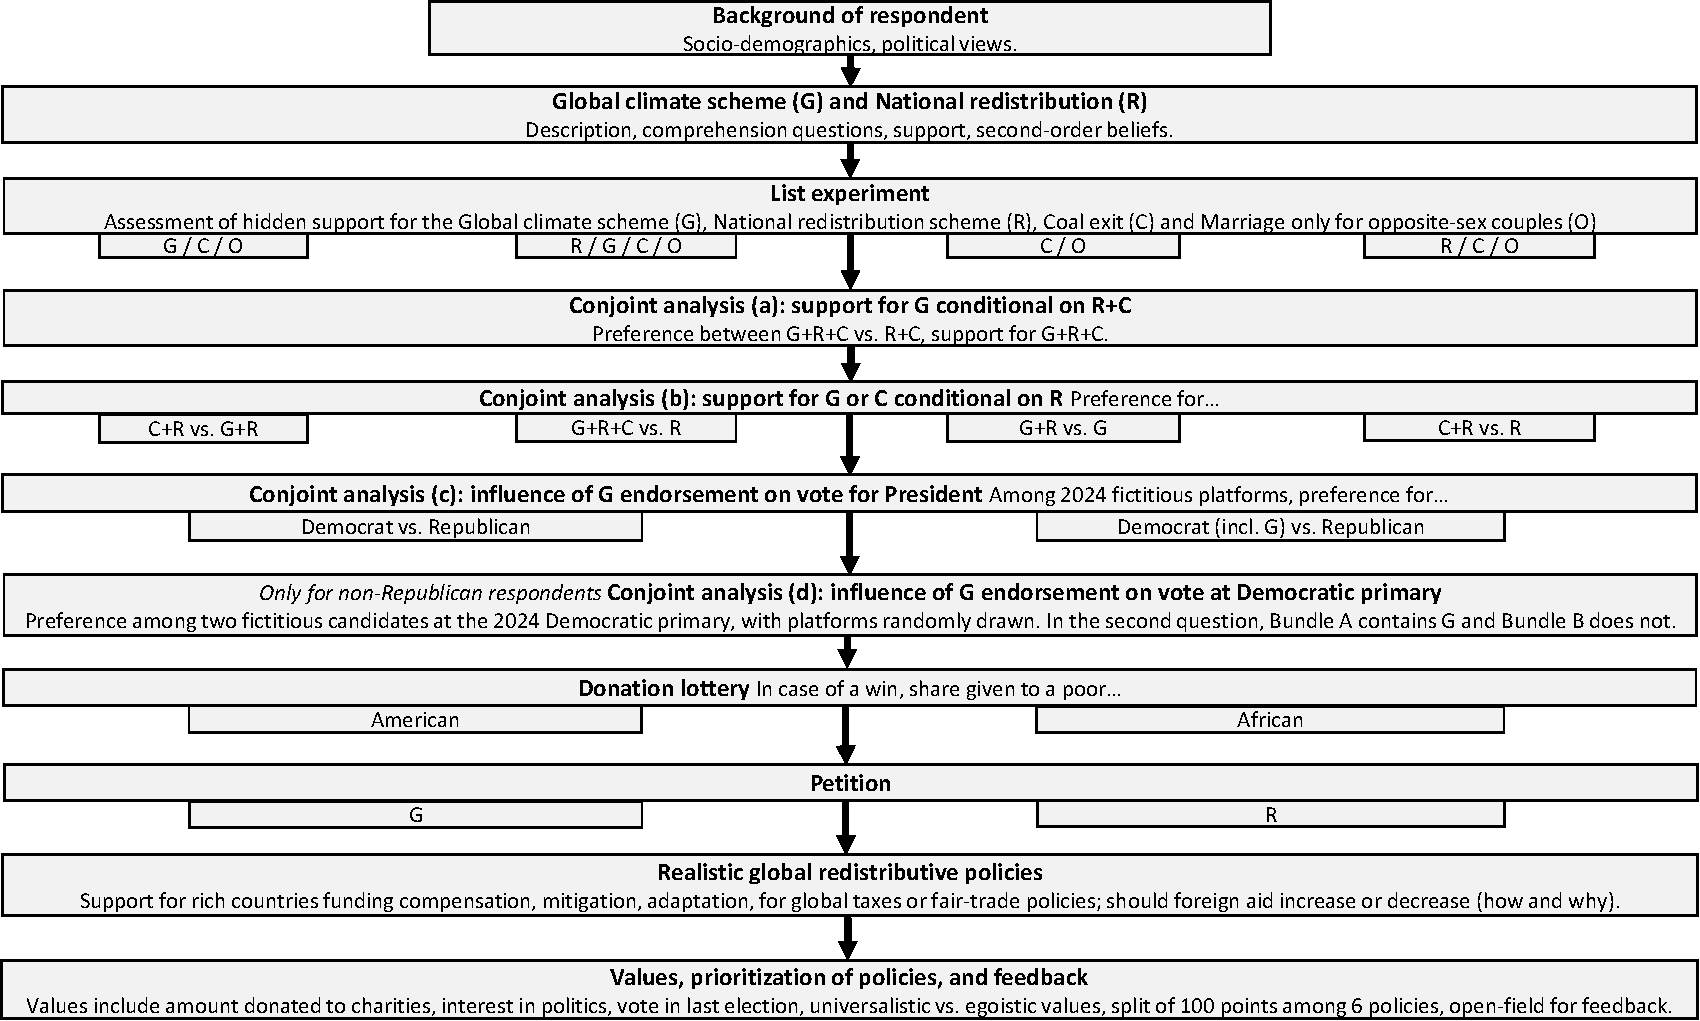
\includegraphics[width=\textwidth]{../questionnaire/survey_flow_US1.pdf}} 
\end{figure}

\subsection*{Socio-demographic characteristics}
\begin{enumerate}[resume] 
\item Welcome to this survey!\\
\\
This survey is \textbf{anonymous} and is conducted \textbf{for research} purposes on a representative sample of 3,000 American people.\\
 \\
It takes \textbf{10 to 15 min} to complete.  \\
 \\
The survey contains lotteries and awards for those who get the correct answer to some understanding questions.\\
If you are attentive and lucky, \textbf{you can win up to \$350} in points. (\href{https://uvafeb.eu.qualtrics.com/WRQualtricsControlPanel/File.php?F=F_cBZAXTgNktGZbee&download=1}{See terms and conditions}).    \\
Please answer every question carefully.  \\
 \\
\textbf{Do you agree to participate in the survey?}
\\ \textit{Yes; No}
\item What is your gender?
\\ \textit{Woman; Man; Other}
\item How old are you?
\\ \textit{Below 18; 18 to 20; 21 to 24; 25 to 29; 30 to 34; 35 to 39; 40 to 44; 45 to 49; 50 to 54; 55 to 59; 60 to 64; 65 to 69; 70 to 74; 75 to 79; 80 to 84; 85 to 89; 90 to 99; 100 or above}
\item What is your ZIP code?%Outcode (the left part of your postcode)?
\item Do you live with your partner (if you have one)?
\\ \textit{Yes; No}
\item How many people are in your household? The household includes: you, the members of your family who live with you, and your dependants. %This excludes flatmates.
\\ \textit{1; 2; 3; 4; 5 or more}
\item What race or ethnicity do you identify with? (Multiple answers are possible) 
\\ \textit{White; Black or African American; Hispanic; Asian; American Indian or Alaskan Native; Natice Hawaiian or Pacific Islander; Other: \{open field\}; Prefer not to say}
\item What is the \textit{annual} gross income of your household (before withholding tax)? This includes all income: wages, self-employment earnings, Social Security benefits, pensions, investment income, welfare payments, and income from other sources. % ~[quartiles thresholds are given for the U.S. ] 
\\ \textit{Less than \$20,000; between \$20,001 and \$35,000; between \$35,001 and \$42,000; between \$42,001 and \$50,000; between \$50,001 and \$65,000; between \$65,001 and \$82,000; between \$82,001 and \$103,000; between \$103,001 and \$130,000; between \$130,001 and \$145,000; between \$145,001 and \$165,000; between \$165,001 and \$250,000; More than \$250,000; I prefer not to answer}
\item What is the highest level of education you have completed? 
\\ \textit{Primary school or less; Eigth grade; Some high school; Regular high school diploma/GED or alternative credential; Some college, no degree; 2-year college degree or associates degree (for example: AA, AS); Bachelor's degree (for example: BA, BS); Master’s degree or above (MA, MS, MEng, MEd, MSW, MBA, MD, DDS, DVM, LLB, JD, PhD); }
\item What is your employment status? \label{item:employment}
\\ \textit{Full-time employed; Part-time employed; Self-employed; Student; Retired; Unemployed (searching for a job); Inactive (not searching for a job)}
\item Are you a homeowner or a tenant? (Multiple answers are possible) 
\\ \textit{Tenant; Owner; Landlord renting out property; Hosted free of charge}
\item ~[Asked if lives with partner] What is the estimated value of your household's assets (in U.S. dollars)?  \\
   \\
Include here all your possessions (home, car, savings, etc.) net of debt. For example, if you own a house worth \$300,000 and you have \$100,000 left to repay on your mortgage, your assets are \$200,000.  \\
  \\
I estimate my household's assets net of debt to be:  \\% ~[Quintiles thresholds are given for the U.S. ]
\\  \textit{Less than \$0 (I have a net debt); Close to \$0; Between \$4,000 and \$120,000; Between \$120,000 and \$380,000; More than \$380,000}
\item ~[Asked if does not live with partner] What is the estimated value of your assets (in U.S. dollars)?   \\
   \\
Include here all your possessions (home, car, savings, etc.) net of debt. For example, if you own a house worth \$300,000 and you have \$100,000 left to repay on your mortgage, your assets are \$200,000.  \\
  \\
  I estimate my assets net of debt to be: \\% ~[Quintiles thresholds are given for the U.S. ]
\\  \textit{Less than \$0 (I have a net debt); Close to \$0; Between \$4,000 and \$60,000; Between \$60,000 and \$190,000; More than \$190,000}
\item What do you consider to be your political affiliation, as of today?
\\ \textit{Republican; Democrat; Independent; Other; Non-Affiliated}
\end{enumerate}

\subsection*{Global climate scheme}
\begin{enumerate}[resume] \item[] In the following, we describe two policies, on which we will survey your opinion. To check that you have attentively read the descriptions,~\textbf{we will ask some understanding questions afterwards: those who get correct answers can win up to \$150}. \\
\textbf{\underbar{Global climate scheme:}}~ At the Paris agreement in 2015, all countries have agreed to contain global warming ``well below +2 $\mathrm{{}^\circ}$C''. To limit global warming to this level,~\textbf{there is a maximum amount of greenhouse gases we can emit globally}.\\
To meet the climate target, a limited number of permits to emit greenhouse gases can be created globally. Polluting firms would be required to buy permits to cover their emissions. Such a policy would~\textbf{make fossil fuel companies pay}~for their emissions and progressively raise the price of fossil fuels.~\textbf{Higher prices would encourage people and companies to use less fossil fuels, reducing greenhouse gas emissions.}\\
In accordance with the principle that each human has an equal right to pollute, the revenues generated by the sale of permits could finance a global basic income.~\textbf{Each adult in the world would receive \$30/month}, thereby lifting out of extreme poverty the 700 million people who earn less than \$2/day.\\
\textbf{The typical American would lose out financially \$85 per month}~(as he or she would face \$115 per month in price increases, which is higher than the \$30 they would receive). The policy could be put in place as soon as countries totaling more than 60\% of global emissions agree on it. Countries that would refuse to take part in the policy could face sanctions (like tariffs) from the rest of the World and would be excluded from the basic income.
\item \label{q:understood_gcs} Who would win or lose financially in the Global climate scheme? [\textit{Figure \ref{fig:understood_each}}] \\
\\
Three respondents with the expected answer will get \$50 in points.
\\ \textit{Typical Americans would win and the 700 million poorest humans would win.; Typical Americans would win and the 700 million poorest humans would lose.; Typical Americans would lose and the 700 million poorest humans would win.; Typical Americans would lose and the 700 million poorest humans would lose.}
\item[[new page\!\!\!]] For your information, the expected answer was \textit{Typical Americans would lose and the 700 million poorest humans would win} from the Global climate scheme. Now, here is the second policy: \\ 
\\
Now, here is the second policy:  \textbf{\underbar{National redistribution scheme:}} This policy would \textbf{increase taxes on the top 5\%} and provide cash transfers to all adults. More precisely, \textbf{each American adult would receive \$85 per month} (that is \$1,000 per year). This would be financed by an increase of the federal income tax on household income in excess of \$315,000 per year, leaving taxes unchanged for income below \$315,000. \underbar{See more details}.
\item \label{q:understood_nr} Who would win or lose financially in the National redistribution? [\textit{Figure \ref{fig:understood_each}}] \\
\\
Three respondents with the expected answer will get \$50 in points.
\\ \textit{Typical Americans would win and the richest Americans would win.; Typical Americans would win and the richest Americans would lose.; Typical Americans would lose and the richest Americans would win.; Typical Americans would lose and the richest Americans would lose.}
\item[[new page\!\!\!]] For your information, the expected answer was \textit{Typical Americans would win and the richest Americans would lose} from the National redistribution scheme. \\ 
\\
To help you with the next question, here is a reminder of the policies:\\
\\
\textbf{\underbar{Global Climate scheme:}}\\ 
To limit global warming and reach the international climate objective, the Global climate scheme would \textbf{impose a maximum amount of greenhouse gases we can emit globally}.\\
It would \textbf{make polluters pay} for their emissions, which in turn would increase fossil fuel prices and discourage polluting activities.\\
The revenues would finance a \textbf{global basic income} of \$30 per month for all humans, lifting out of extreme poverty the poorest billion people.\\
Considering the basic income and the fuel price increases, \textbf{the typical American would lose out financially \$85 per month}.\\
\\
\textbf{\underbar{National redistribution scheme:}} This policy would \textbf{increase taxes on the top 5\%} and provide cash transfers to all adults. More precisely, \textbf{each American would receive \$85 per month}. This would be financed by an increase of the federal income tax on household income in excess of \$315,000 per year, leaving taxes unchanged for income below \$315,000 per year.
\item \label{q:understood_both} If both the Global climate scheme and the National redistribution scheme are implemented, how would a typical American be financially affected? [\textit{Figure \ref{fig:understood_each}}] \\
Three respondents with the expected answer will get \$50 in points.
\\ \textit{A typical American would lose out financially.; A typical American would neither gain nor lose.; A typical American would gain financially.}
\item[[new page\!\!\!]] For your information, the expected answer was that \textit{A typical American would neither gain nor lose} from both schemes combined. Now, here are the last two policies:\\
\\
\textbf{\underbar{Coal exit:}} To reduce CO2~emissions, this policy would require all U.S. coal power plants to be phased out by 2030. Coal would be replaced by renewable sources like wind and solar panels as well as stronger reliance on gas power plants.\\
\\
\textbf{\underbar{Marriage only for opposite-sex couples:}}\\
This policy is a proposed amendment to the U.S. Constitution that would legally define marriage as a union of one man and one woman.\\
\\
Now, we will ask your opinion on the four policies.\\
\underbar{Click here for the reminder of the first two policies.} [\textit{Clicking displays the previous summarized descriptions.}]
\item \label{q:gcs_support} Do you support the Global climate scheme? [\textit{Figure \ref{fig:support_binary}}]
\\ \textit{Yes; No}
\item \label{q:gcs_belief} According to you, what percentage of Americans answer Yes to the previous question? [\textit{Figure \ref{fig:belief}}]\\
The three people who are closest to the true value get \$50 in panel points.
\\ \textit{Percentage of Americans in favor of Global climate scheme} [slider from 0 to 100]
\item \label{q:nr_support} Do you support the National redistribution scheme? [\textit{Figure \ref{fig:support_binary}}]
\\ \textit{Yes; No}
\item \label{q:nr_belief} According to you, what percentage of Americans answer Yes to the previous question? [\textit{Figure \ref{fig:belief}}]\\
The three people who are closest to the true value get \$50 in panel points.
\\ \textit{Percentage of Americans in favor of National redistribution } [slider from 0 to 100]
% \item ~[Random branch (list\_exp)] \label{q:list_exp_1} Beware, this question is quite unusual. Among the policies below, \textbf{how many} do you support?
% \begin{itemize} 
%     \item Global climate scheme 
%     \item Coal exit  
%     \item Marriage only for opposite-sex couples
% \end{itemize}
% \textit{0; 1; 2; 3}
% \item ~[Random branch (list\_exp)] Beware, this question is quite unusual. Among the policies below, \textbf{how many} do you support?
% \begin{itemize} 
%     \item Global climate scheme 
%     \item National redistribution scheme
%     \item Coal exit  
%     \item Marriage only for opposite-sex couples
% \end{itemize}
% \textit{0; 1; 2; 3; 4}
% \item ~[Random branch (list\_exp)] Beware, this question is quite unusual. Among the policies below, \textbf{how many} do you support?
% \begin{itemize} 
%     \item Coal exit  
%     \item Marriage only for opposite-sex couples
% \end{itemize}
% \textit{0; 1; 2}
% \item ~[Random branch (list\_exp)] \label{q:list_exp_4} Beware, this question is quite unusual. Among the policies below, \textbf{how many} do you support?
% \begin{itemize} 
%     \item National redistribution scheme 
%     \item Coal exit  
%     \item Marriage only for opposite-sex couples
% \end{itemize}
% \textit{0; 1; 2; 3}
\item \label{q:list_exp} Beware, this question is quite unusual. Among the policies below, \textbf{how many} do you support? [\textit{Figure \ref{fig:list_exp}}]\\
~[\textit{Four random branches. Branch GCS/NR/C/O}] \\
\begin{itemize} \vspace{-1em}
    \item Global climate scheme 
    \item National redistribution scheme
    \item Coal exit  
    \item Marriage only for opposite-sex couples
\end{itemize}
\textit{0; 1; 2; 3; 4}\\
\\
~[\textit{Branch GCS/C/O}] \\
\begin{itemize}  \vspace{-1em}
    \item Global climate scheme 
    \item Coal exit  
    \item Marriage only for opposite-sex couples
\end{itemize}
\textit{0; 1; 2; 3}\\
\\
~[\textit{Branch C/O}] \\
\begin{itemize}  \vspace{-1em}
    \item Coal exit  
    \item Marriage only for opposite-sex couples
\end{itemize}
\textit{0; 1; 2}\\
\\
~[\textit{Branch NR/C/O}] \\
\begin{itemize}  \vspace{-1em}
    \item National redistribution scheme 
    \item Coal exit  
    \item Marriage only for opposite-sex couples
\end{itemize}
\textit{0; 1; 2; 3}
\end{enumerate}

\subsection*{Conjoint analyses}
\begin{enumerate}[resume]
\item \label{q:conjoint_a} Among the two following bundles of policies, which one would you prefer? [\textit{Figure \ref{fig:conjoint}}] \\ 
Note that for each bundle, all policies of the bundle would be implemented at the same time.\\
    \begin{tabular}{@{\extracolsep{5pt}}|c|c|} 
        \hline \\[-1.8ex] 
        \textbf{Bundle A} & \textbf{Bundle B}  \\ \hline \\[-1.8ex]
        Coal exit & Coal exit \\ 
        National redistribution scheme & National redistribution scheme \\ 
        Global climate scheme &  \\ 
        \hline
    \end{tabular}\\ 
\\ \textit{Bundle A; Bundle B}
\item \label{q:crg_support} Do you support Bundle A (combining Coal exit, the National redistribution scheme, and the Global climate scheme)?[\textit{Figure \ref{fig:support_binary}}]
\\ \textit{Yes; No}
% \item ~[new page] [Random branch (conjoint analysis b.)] \label{q:conjoint_b_1} Among the two following bundles of policies, which one would you prefer? \\ 
% Note that for each bundle, all policies of the bundle would be implemented at the same time.\\
%     \begin{tabular}{@{\extracolsep{5pt}}|c|c|} 
%         \hline \\[-1.8ex] 
%         \textbf{Bundle A} & \textbf{Bundle B}  \\ \hline \\[-1.8ex]
%         Coal exit & Global climate scheme \\ 
%         National redistribution scheme & National redistribution scheme \\ 
%         \hline 
%     \end{tabular}\\ 
% \\ \textit{Bundle A; Bundle B}
% \item ~[new page] [Random branch (conjoint analysis b.)] Among the two following bundles of policies, which one would you prefer? \\ 
% Note that for each bundle, all policies of the bundle would be implemented at the same time.\\
%     \begin{tabular}{@{\extracolsep{5pt}}|c|c|} 
%         \hline \\[-1.8ex] 
%         \textbf{Bundle A} & \textbf{Bundle B}  \\ \hline \\[-1.8ex]
%         National redistribution scheme & National redistribution scheme \\ 
%          & Coal exit \\ 
%          & Global climate scheme \\ 
%         \hline
%     \end{tabular}\\ 
% \\ \textit{Bundle A; Bundle B}
% \item ~[new page] [Random branch (conjoint analysis b.)] Among the two following bundles of policies, which one would you prefer? \\ 
% Note that for each bundle, all policies of the bundle would be implemented at the same time.\\
%     \begin{tabular}{@{\extracolsep{5pt}}|c|c|} 
%         \hline \\[-1.8ex] 
%         \textbf{Bundle A} & \textbf{Bundle B}  \\ \hline \\[-1.8ex]
%         National redistribution scheme & National redistribution scheme \\ 
%         Global climate scheme &  \\ 
%         \hline 
%     \end{tabular}\\ 
% \\ \textit{Bundle A; Bundle B}
% \item ~[new page] [Random branch (conjoint analysis b.)] \label{q:conjoint_b_4} Among the two following bundles of policies, which one would you prefer? \\ 
% Note that for each bundle, all policies of the bundle would be implemented at the same time.\\
%     \begin{tabular}{@{\extracolsep{5pt}}|c|c|} 
%         \hline \\[-1.8ex] 
%         \textbf{Bundle A} & \textbf{Bundle B}  \\ \hline \\[-1.8ex]
%         National redistribution scheme & National redistribution scheme \\ 
%         Coal exit &  \\ 
%         \hline
%     \end{tabular}\\ 
% \\ \textit{Bundle A; Bundle B} 
\item ~[new page] \label{q:conjoint_b} Among the two following bundles of policies, which one would you prefer? [\textit{Figure \ref{fig:conjoint}}]\\ 
Note that for each bundle, all policies of the bundle would be implemented at the same time.\\
~[\textit{Four random branches. Branch C + NR vs. GCS + NR}]\\
\begin{tabular}{@{\extracolsep{5pt}}|c|c|} 
    \hline \\[-1.8ex] 
    \textbf{Bundle A} & \textbf{Bundle B}  \\ \hline \\[-1.8ex]
    Coal exit & Global climate scheme \\ 
    National redistribution scheme & National redistribution scheme \\ 
    \hline 
\end{tabular}\\ 
\\
~[\textit{Branch NR vs. NR + C + GCS}]\\
\begin{tabular}{@{\extracolsep{5pt}}|c|c|} 
    \hline \\[-1.8ex] 
    \textbf{Bundle A} & \textbf{Bundle B}  \\ \hline \\[-1.8ex]
    National redistribution scheme & National redistribution scheme \\ 
     & Coal exit \\ 
     & Global climate scheme \\ 
    \hline
\end{tabular}\\ 
\\
~[\textit{Branch NR + GCS vs. NR}]\\
\begin{tabular}{@{\extracolsep{5pt}}|c|c|} 
    \hline \\[-1.8ex] 
    \textbf{Bundle A} & \textbf{Bundle B}  \\ \hline \\[-1.8ex]
    National redistribution scheme & National redistribution scheme \\ 
    Global climate scheme &  \\ 
    \hline 
\end{tabular}\\ 
\\
~[\textit{Branch NR + C vs. NR}]\\
    \begin{tabular}{@{\extracolsep{5pt}}|c|c|} 
        \hline \\[-1.8ex] 
        \textbf{Bundle A} & \textbf{Bundle B}  \\ \hline \\[-1.8ex]
        National redistribution scheme & National redistribution scheme \\ 
        Coal exit &  \\ 
        \hline
    \end{tabular}\\ 
\\ \textit{Bundle A; Bundle B} 
\item ~[new page] \label{q:conjoint_c} Imagine if the Democratic and Republican presidential candidates in 2024 campaigned with the following policies in their platforms.\\
\\
Which of these candidates would you vote for? [\textit{Figure \ref{fig:conjoint}}]\\
    ~[\textit{Two random branches: with and without the final row.}] \\
    \begin{tabular}{|>{\centering\arraybackslash}p{7cm}|>{\centering\arraybackslash}p{7cm}|}
    \hline \\[-1.8ex] 
        \textbf{Democrat} & \textbf{Republican}  \\ \hline \\[-1.8ex]
        Increase corporate income tax rate from 21\% to 28\% & Decrease the payroll tax \\ 
        Coal exit & Permit completion of the Keystone pipeline \\ 
        Trillion dollar investment in childcare, healthcare, education and housing & Withdrawal of the Paris agreement \\ 
        \$15 minimum wage & Marriage only for opposite-sex couples \\ 
        National redistribution scheme & Strict enforcement of immigration and border legislation \\ 
        ~[Global climate scheme / \textit{no row}] & [ / \textit{no row}]\\ 
        \hline
    \end{tabular}\\ 
\\ \textit{Democrat; Republican; None of them}
\item ~[new page] [Asked only to non-Republicans] \label{q:conjoint_r} Imagine that at the 2024 Democratic party presidential primaries, the two main candidates campaign with the following key policies in their platforms.\\
\\
Which of these candidates do you prefer? [\textit{Figures \ref{fig:conjoint} and \ref{fig:ca_r}}]\\
\begin{tabular}{@{\extracolsep{5pt}}|c|c|c|} 
    \hline \\[-1.8ex] 
    & \textbf{Candidate A} & \textbf{Candidate B}  \\ \hline \\[-1.8ex]
    ~[Policy field in random order] & [Random policy] & [Random policy] \\ 
    ~[Policy field in random order] & [Random policy] & [Random policy] \\ 
    ~[Policy field in random order] & [Random policy] & [Random policy] \\ 
    ~[Policy field in random order] & [Random policy] & [Random policy] \\ 
    ~[Policy field in random order] & [Random policy] & [Random policy] \\ 
    \hline 
\end{tabular} 
\\ \textit{Candidate A; Candidate B}
\item ~[new page] [Asked only to non-Republicans] \label{q:conjoint_d} Imagine that at the 2024 Democratic party presidential primaries, the two main candidates campaign with the following key policies in their platforms.\\
\\
Which of these candidates do you prefer? [\textit{Figure \ref{fig:conjoint}}]\\
\begin{tabular}{@{\extracolsep{5pt}}|c|c|c|} 
    \hline \\[-1.8ex] 
     & \textbf{Candidate A} & \textbf{Candidate B}  \\ \hline \\[-1.8ex]
    ~[Policy field in random order] & [Random policy] & [Random policy] \\ 
    ~[Policy field in random order] & [Random policy] & [Random policy] \\ 
    ~[Policy field in random order] & [Random policy] & [Random policy] \\ 
    ~[Policy field in random order] & [Random policy] & [Random policy] \\ 
    \textbf{Foreign policy} & Global climate scheme & - \\ 
    \hline 
\end{tabular} 
\\ \textit{Candidate A; Candidate B}
\end{enumerate}

\subsection*{Donation lottery}
\begin{enumerate}[resume] \item Please select ``A little'' (this is a test to see if you are paying attention).
\\ \textit{Not at all; A little; A lot; A great deal}
\item ~[\textit{Two random branches}] \label{q:donation} By taking this survey, you are automatically entered into a lottery to win \$100 in panel points. This lottery is unrelated to the previous ones that rewarded answers' accuracy. In a few days you will know whether you have been selected in the lottery. The payment will be made to you in the same way as your compensation for this survey, so no further action is required on your part.\\
\\
Should you be selected in the lottery, you can also donate a part of this additional compensation to [American / African] people living in poverty through the charity GiveDirectly. The charity GiveDirectly provides small amounts of cash to people in need in [the U.S / Africa].\\
\\
\textbf{In case you are winner of the lottery, what share of the \$100 would you donate to [American / African] people living in poverty through GiveDirectly?}  [\textit{Figure \ref{fig:donation}}]
\\ \textit{Amount donated to [American / African] people in need (in \$)} [slider from 0 to 100]
\item Please select ``A little'' (this is a test to see if you are paying attention).
\\ \textit{Not at all; A little; A lot; A great deal}
% \item ~[Random branch (donation)] \label{q:donation_2} By taking this survey, you are automatically entered into a lottery to win \$100 in panel points. This lottery is unrelated to the previous ones that rewarded answers' accuracy. In a few days you will know whether you have been selected in the lottery. The payment will be made to you in the same way as your compensation for this survey, so no further action is required on your part.\\
% \\
% Should you be selected in the lottery, you can also donate a part of this additional compensation to African people living in poverty through the charity GiveDirectly. The charity GiveDirectly provides small amounts of cash to people in need in Africa.\\
% \\
% \textbf{In case you are winner of the lottery, what share of the \$100 would you donate to African people living in poverty through GiveDirectly?}
% \\ \textit{Amount donated to African people in need (in \$)} [slider from 0 to 100]
\end{enumerate}

\subsection*{Petition}
\begin{enumerate}[resume] \item ~[\textit{Two random branches}] \label{q:petition} Would you be willing to sign a petition for the [Global climate / National redistribution] scheme?  [\textit{Figure \ref{fig:petition}}]\\
\\
As soon as the survey is complete, we will send the results to the U.S. President's office, informing him what share of American people are willing to endorse the [Global climate / National redistribution] scheme. (You will NOT be asked to sign, only your answer here is required and remains anonymous.) 
\textit{Yes; No}
% \item Would you be willing to sign a petition for the Global climate scheme? \\
% \\
% As soon as the survey is complete, we will send the results to the U.S. President's office, informing him what share of American people are willing to endorse the Global climate scheme. (You will NOT be asked to sign, only your answer here is required and remains anonymous.) 
% \textit{Yes; No}
% \item Would you be willing to sign a petition for the National redistribution scheme? \\
% \\
% As soon as the survey is complete, we will send the results to the U.S. President's office, informing him what share of American people are willing to endorse the National redistribution scheme. (You will NOT be asked to sign, only your answer here is required and remains anonymous.) 
% \textit{Yes; No}
\end{enumerate}

\subsection*{Other policies}
\begin{enumerate}[resume] \item \label{q:climate_policies} The following policies are discussed  at international negotiations on how to deal with climate change. [\textit{Figure \ref{fig:support_likert}}]\\
\\
Do you support or oppose the following policies?
\begin{itemize}
    \item Payments from high-income countries to compensate low-income countries for climate damages 
    \item High-income countries funding renewable energy in low-income countries
    \item High-income countries contributing \$100 billion per year to help low-income countries adapt to climate change
\end{itemize}
\textit{Strongly oppose; Somewhat oppose; Neither support nor oppose; Somewhat support; Strongly support}
\item \label{q:other_policies} Do you support or oppose the following global policies? [\textit{Figure \ref{fig:support_likert}}]
\begin{itemize}
    \item Cancellation of low-income countries' public debt 
    \item Democratise international institutions (UN, IMF) by making a country's voting right proportional to its population 
    \item Removing tariffs on imports from low-income countries
    \item A minimum wage in all countries at 50\% of local median wage
    \item Fight tax evasion by creating a global financial register to record ownership of all assets
    \item A maximum wealth limit of \$10 billion for each human 
\end{itemize}
\textit{Strongly oppose; Somewhat oppose; Neither support nor oppose; Somewhat support; Strongly support}
\item \label{q:foreign_aid_raise_support} Currently, 0.4\% of U.S. government spending (that is, 0.2\% of U.S. GDP) is spent on foreign aid to reduce poverty in low-income countries. [\textit{Figure \ref{fig:foreign_aid_raise_support}}]\\
\\
Do you support the U.S. transferring more money to low-income countries?
\\ \textit{Yes, U.S. foreign aid should be increased.; Yes, but only if some conditions are met.; No, U.S. foreign aid should remain stable.; No, U.S. foreign aid should be reduced.}
\item ~[Asked only if \textit{Yes, but only if some conditions are met.} is chosen] \label{q:foreign_aid_condition} What conditions should be required for the U.S. to increase its foreign aid? (Multiple answers possible) [\textit{Figure \ref{fig:foreign_aid_condition}}]
\\ \textit{That recipient countries comply with climate targets and human rights.; That recipient countries cooperate to fight illegal migrations.; That other high-income countries also increase their foreign aid.; That this is financed by increased taxes on millionaires.; That we can be sure the aid reaches people in need and money is not diverted.; Other: [open field]}
\item ~[Asked only if \textit{No, U.S. foreign aid should remain stable.} or \textit{No, U.S. foreign aid should be reduced.} is chosen] \label{q:foreign_aid_no} Why do you oppose the U.S. increasing its foreign aid? (Multiple answers possible) [\textit{Figure \ref{fig:foreign_aid_no}}]
\\ \textit{Aid perpetuates poverty as it makes people feel less responsible for themselves.; Aid is not effective as most of it is diverted.; Aid is a pressure tactic for high-income countries that prevents low-income countries from developing freely.; The U.S. is not responsible for what happens in other countries.; Charity begins at home: there is already a lot to do to support the American people in need.; Other: [open field]}
\end{enumerate}

\subsection*{Values and politics}
\begin{enumerate}[resume] \item \label{q:negotiation} In international climate negotiations, would you prefer U.S. diplomats to defend U.S. interests or global justice? [\textit{Figure \ref{fig:negotiation}}]
\\ \textit{U.S. interests, even if it goes against global justice; U.S. interests, to the extent it respects global justice; ndifferent or don't know; Global justice, to the extent it respects U.S. interests; Global justice, even if it goes against U.S. interests}
\item How much did you give to charities in 2022?
\\ \textit{I did not make donations to charities last year.; Less than \$100.; Between \$101 and \$500.; Between \$501 and \$1,000.; Between \$1,001 and \$5,000.; More than \$5,000.}
\item To what extent are you interested in politics?
\\ \textit{Not at all; A little; Moderately; A lot; A great deal}
\item Where would you rate yourself on a scale of 1 to 5, where 1 means you think the government should do only those things necessary to provide the most basic government functions, and 5 means you think the government should take active steps in every area it can to try and improve the lives of its citizens?
\\ \textit{Desired involvement of government} [slider from 1 to 5]
\item \textbf{On economic policy matters}, where do you see yourself on a scale of 1 to 5, where 1 is Left (favoring equality and government interventions) and 5 is Right (favoring free competition and little government intervention)?
\\ \textit{Left (1) to Right (5) on economic issues} [slider from 1 to 5]
\item Did you vote in the 2020 U.S. presidential election? \label{item:election}
\\ \textit{Yes; No: I didn't have the right to vote in the U.S.; Prefer not to say}
\item ~[Asked if voted] Which candidate did you vote for in the 2020 U.S. presidential election?
\\ \textit{Biden; Trump; Jorgensen; Hawkins; Prefer not to say}
\item ~[Asked if did not vote] Even if you did not vote in the 2020 U.S. presidential election, please indicate the candidate that you were most likely to have voted for or who represents your views more closely.
\\ \textit{Biden; Trump; Jorgensen; Hawkins; Prefer not to say}
\item \label{q:problem} To what extent do you think the following issues are a problem? [\textit{Figure \ref{fig:problem}}]
\begin{itemize}
    \item Income inequality in the U.S. 
    \item Climate change
    \item Global poverty
\end{itemize}
\textit{Not an important issue for me; An issue but there are other priorities; An issue but we already do what we can; An important issue, we should do more; One of the most pressing issue of our time}
\item \label{q:group_defended_agg} What group do you defend when you vote? [\textit{Figure \ref{fig:group_defended_agg}}]
\\ \textit{Sentient beings (humans and animals); Humans; Americans; People sharing my culture or religion; My State; My town; My relatives and/or colleagues; My family and myself}
\end{enumerate}

\subsection*{Prioritization}
\begin{enumerate}[resume] \item \label{q:points_us} In this question, you have 100 points that you can allocate to different policies. The more you give points to a policy, the more you support it.\\ 
   \\
    How do you allocate the points among the following policies? [\textit{Figure \ref{fig:points_us}}]  \\
    \\
    You can adjust the number of points either using the slider or entering the number of your choice on the right-hand-side. \textbf{The sum of points must equal exactly 100}. By pushing the last slider to the right, the total will automatically adjust to 100. Please read the 6 options before making your choice.
\begin{itemize}
    \item Student loan forgiveness
    \item \$15 minimum wage 
    \item Universal childcare/pre-K 
    \item Funding affordable housing 
    \item Expanding the Supreme Court 
    \item Handgun ban 
    \item Making abortion a right at the federal level 
    \item Coal exit 
    \item Trillion dollar investment in clean transportation infrastructure and building insulation 
    \item Ban the sale of new combustion-engine cars by 2030 
    \item National redistribution scheme 
    \item Wealth tax 
    \item Increase corporate income tax rate from 21\% to 28\% 
    \item Global climate scheme 
    \item Global tax on millionaires 
    \item Global democratic assembly on climate change 
    \item Doubling foreign aid 
\end{itemize}
[slider from 0 to 100]
\end{enumerate}

\subsection*{Feedback}
\begin{enumerate}[resume]
\item Do you feel that this survey was politically biased?
\\ \textit{Yes, left-wing biased; Yes, right-wing biased; No, I do not feel it was biased}
\item The survey is nearing completion. You can now enter any comments, thoughts or suggestions in the field below.
\\ ~[open-ended field]
\item Lastly, are you interested to be interviewed by a researcher (through videoconferencing) for 30 min? \\
\\
This is totally optional and will not be rewarded.
\\ \textit{Yes; No}
\end{enumerate}

\clearpage
\section{Representativeness of the surveys}\label{app:representativeness}


\begin{table}[h!]
    \caption{Sample representativeness of the complementary surveys.} \label{tab:representativeness_waves}
    \makebox[\textwidth][c]{
        \resizebox*{!}{.80\textheight}{% 73 without notes cf. https://tex.stackexchange.com/questions/13809/resizing-a-table-by-textheight 
        
\begin{tabular}[t]{llllllllll}
\toprule
\multicolumn{1}{c}{} & \multicolumn{3}{c}{US1} & \multicolumn{3}{c}{US2} & \multicolumn{3}{c}{EU} \\
\cmidrule(l{3pt}r{3pt}){2-4} \cmidrule(l{3pt}r{3pt}){5-7} \cmidrule(l{3pt}r{3pt}){8-10}
  & Pop. & Sample & \makecell{Weighted\\sample} & Pop. & Sample & \makecell{Weighted\\sample} & Pop. & Sample & \makecell{Weighted\\sample}\\
\midrule
Sample size &  & 3,000 & 3,000 &  & 516 & 516 &  & 2,979 & 2,979\\
\addlinespace
Gender: Woman & 0.51 & 0.52 & 0.51 & 0.51 & 0.65 & 0.56 & 0.51 & 0.49 & 0.51\\
Gender: Man & 0.49 & 0.47 & 0.49 & 0.49 & 0.34 & 0.44 & 0.49 & 0.51 & 0.49\\
\addlinespace
Income\_quartile: 1 & 0.25 & 0.27 & 0.25 & 0.25 & 0.53 & 0.35 & 0.25 & 0.28 & 0.25\\
Income\_quartile: 2 & 0.25 & 0.24 & 0.25 & 0.25 & 0.31 & 0.31 & 0.25 & 0.23 & 0.25\\
Income\_quartile: 3 & 0.25 & 0.25 & 0.25 & 0.25 & 0.13 & 0.23 & 0.25 & 0.25 & 0.25\\
Income\_quartile: 4 & 0.25 & 0.23 & 0.25 & 0.25 & 0.04 & 0.11 & 0.25 & 0.24 & 0.25\\
\addlinespace
Age: 18-24 & 0.12 & 0.12 & 0.12 & 0.12 & 0.09 & 0.11 & 0.10 & 0.11 & 0.10\\
Age: 25-34 & 0.18 & 0.15 & 0.18 & 0.18 & 0.19 & 0.19 & 0.15 & 0.17 & 0.15\\
Age: 35-49 & 0.24 & 0.25 & 0.24 & 0.24 & 0.29 & 0.25 & 0.24 & 0.25 & 0.24\\
Age: 50-64 & 0.25 & 0.27 & 0.25 & 0.25 & 0.27 & 0.27 & 0.26 & 0.25 & 0.26\\
Age: 65+ & 0.21 & 0.21 & 0.21 & 0.21 & 0.16 & 0.18 & 0.25 & 0.23 & 0.25\\
\addlinespace
Diploma\_25\_64: Below upper secondary & 0.06 & 0.02 & 0.05 & 0.06 & 0.06 & 0.06 & 0.13 & 0.14 & 0.13\\
Diploma\_25\_64: Upper secondary & 0.28 & 0.25 & 0.28 & 0.28 & 0.41 & 0.33 & 0.23 & 0.19 & 0.23\\
Diploma\_25\_64: Post secondary & 0.34 & 0.40 & 0.34 & 0.34 & 0.30 & 0.32 & 0.29 & 0.33 & 0.29\\
\addlinespace
Race: White only & 0.60 & 0.67 & 0.61 & 0.60 & 0.14 & 0.40 &  &  & \\
Race: Hispanic & 0.18 & 0.15 & 0.19 & 0.18 & 0.46 & 0.30 &  &  & \\
Race: Black & 0.13 & 0.16 & 0.14 & 0.13 & 0.37 & 0.22 &  &  & \\
\addlinespace
Region: Northeast & 0.17 & 0.20 & 0.17 & 0.17 & 0.16 & 0.18 &  &  & \\
Region: Midwest & 0.21 & 0.22 & 0.21 & 0.21 & 0.15 & 0.19 &  &  & \\
Region: South & 0.38 & 0.39 & 0.38 & 0.38 & 0.47 & 0.45 &  &  & \\
Region: West & 0.24 & 0.20 & 0.24 & 0.24 & 0.22 & 0.18 &  &  & \\
\addlinespace
Urban: TRUE & 0.73 & 0.78 & 0.74 & 0.73 & 0.83 & 0.74 &  &  & \\
\addlinespace
Employment\_18\_64: Inactive & 0.20 & 0.16 & 0.16 & 0.20 & 0.19 & 0.15 & 0.17 & 0.15 & 0.15\\
Employment\_18\_64: Unemployed & 0.02 & 0.07 & 0.08 & 0.02 & 0.15 & 0.11 & 0.03 & 0.05 & 0.05\\
\addlinespace
Vote: Left & 0.32 & 0.47 & 0.45 & 0.32 & 0.53 & 0.48 & 0.30 & 0.32 & 0.32\\
Vote: Center-right or Right & 0.30 & 0.31 & 0.31 & 0.30 & 0.15 & 0.23 & 0.28 & 0.32 & 0.32\\
Vote: Far right &  &  &  &  &  &  & 0.10 & 0.10 & 0.10\\
\addlinespace
Country: FR &  &  &  &  &  &  & 0.24 & 0.24 & 0.24\\
Country: DE &  &  &  &  &  &  & 0.33 & 0.33 & 0.33\\
Country: ES &  &  &  &  &  &  & 0.18 & 0.18 & 0.18\\
Country: UK &  &  &  &  &  &  & 0.25 & 0.25 & 0.25\\
\addlinespace
Urbanity: Cities &  &  &  &  &  &  & 0.43 & 0.49 & 0.43\\
Urbanity: Towns and suburbs &  &  &  &  &  &  & 0.33 & 0.32 & 0.33\\
Urbanity: Rural &  &  &  &  &  &  & 0.25 & 0.19 & 0.25\\
\bottomrule
\end{tabular}
        }
    }
    {\footnotesize \textit{Note}: This table displays summary statistics of the samples alongside actual population frequencies. %For \textit{Vote}, we regroup candidates or parties into three broad categories and we take abstention into account (but omit this category). 
    %For \textit{Inactivity rate (15-64)}, the sample statistics include the share of respondents aged between 15 and 64 years old who indicated being either ``\textit{Inactive (not searching for a job)},'' a ``\textit{Student},'' or ``\textit{Retired}.'' For \textit{Unemployment rate (15-64)}, the sample statistics include the share of respondents aged between 15 and 64 years old who indicated being ``\textit{Unemployed (searching for a job)}'', (`\textit{Unemployed (searching for a job)},'' ``\textit{Full-time employed},'' ``\textit{Part-time employed},'' or ``\textit{Self-employed}''). For	\textit{Employment rate (15-64)}, the sample statistics include the share of respondents aged between 15 and 64 years old who indicated being either ``\textit{Full-time employed},'' ``\textit{Part-time employed},'' or ``\textit{Self-employed}.'' 
    Detailed sources for each variable and country population frequencies, as well as the definitions of regions, diploma, urbanity, employment, and vote are available in % TODO Appendix \ref{app:sources}.
    } % TODO add hline before Urbanity, move Country/Urbanity above and add in Notes that quotas are those above the line
\end{table}

\begin{table}[h]
    \caption{Sample representativeness for each European country.} \label{tab:representativeness_EU}
    \makebox[\textwidth][c]{
        \resizebox*{!}{.50\textheight}{% 73 without notes cf. https://tex.stackexchange.com/questions/13809/resizing-a-table-by-textheight 
        
\begin{tabular}[t]{lllllllllllll}
\toprule
\multicolumn{1}{c}{} & \multicolumn{3}{c}{FR} & \multicolumn{3}{c}{DE} & \multicolumn{3}{c}{ES} & \multicolumn{3}{c}{UK} \\
\cmidrule(l{3pt}r{3pt}){2-4} \cmidrule(l{3pt}r{3pt}){5-7} \cmidrule(l{3pt}r{3pt}){8-10} \cmidrule(l{3pt}r{3pt}){11-13}
  & Pop. & Sam. & \makecell{Wght.\\sam.} & Pop. & Sam. & \makecell{Wght.\\sam.} & Pop. & Sam. & \makecell{Wght.\\sam.} & Pop. & Sam. & \makecell{Wght.\\sam.}\\
\midrule
Sample size &  & 729 & 729 &  & 979 & 979 &  & 543 & 543 &  & 749 & 749\\
\addlinespace
Gender: Woman & 0.52 & 0.50 & 0.52 & 0.51 & 0.52 & 0.51 & 0.51 & 0.53 & 0.51 & 0.50 & 0.43 & 0.50\\
Gender: Man & 0.48 & 0.50 & 0.48 & 0.49 & 0.48 & 0.49 & 0.49 & 0.47 & 0.49 & 0.50 & 0.57 & 0.50\\
\addlinespace
Income\_quartile: 1 & 0.25 & 0.31 & 0.25 & 0.25 & 0.29 & 0.25 & 0.25 & 0.27 & 0.25 & 0.25 & 0.26 & 0.25\\
Income\_quartile: 2 & 0.25 & 0.17 & 0.25 & 0.25 & 0.25 & 0.25 & 0.25 & 0.31 & 0.25 & 0.25 & 0.19 & 0.25\\
Income\_quartile: 3 & 0.25 & 0.19 & 0.25 & 0.25 & 0.28 & 0.25 & 0.25 & 0.26 & 0.25 & 0.25 & 0.26 & 0.25\\
Income\_quartile: 4 & 0.25 & 0.33 & 0.25 & 0.25 & 0.18 & 0.25 & 0.25 & 0.17 & 0.25 & 0.25 & 0.28 & 0.25\\
\addlinespace
Age: 18-24 & 0.12 & 0.12 & 0.12 & 0.09 & 0.14 & 0.09 & 0.08 & 0.09 & 0.08 & 0.10 & 0.07 & 0.10\\
Age: 25-34 & 0.15 & 0.14 & 0.15 & 0.15 & 0.17 & 0.15 & 0.12 & 0.16 & 0.12 & 0.17 & 0.20 & 0.17\\
Age: 35-49 & 0.24 & 0.31 & 0.24 & 0.22 & 0.26 & 0.22 & 0.28 & 0.25 & 0.28 & 0.24 & 0.18 & 0.24\\
Age: 50-64 & 0.24 & 0.19 & 0.24 & 0.28 & 0.23 & 0.28 & 0.27 & 0.28 & 0.27 & 0.25 & 0.30 & 0.25\\
Age: 65+ & 0.25 & 0.24 & 0.25 & 0.26 & 0.21 & 0.26 & 0.25 & 0.22 & 0.25 & 0.24 & 0.25 & 0.24\\
\addlinespace
Diploma\_25\_64: Below upper secondary & 0.11 & 0.19 & 0.11 & 0.10 & 0.14 & 0.10 & 0.24 & 0.16 & 0.25 & 0.12 & 0.09 & 0.12\\
Diploma\_25\_64: Upper secondary & 0.26 & 0.16 & 0.26 & 0.27 & 0.20 & 0.27 & 0.16 & 0.15 & 0.16 & 0.21 & 0.23 & 0.21\\
Diploma\_25\_64: Post secondary & 0.26 & 0.30 & 0.26 & 0.29 & 0.31 & 0.29 & 0.28 & 0.38 & 0.27 & 0.33 & 0.36 & 0.33\\
\addlinespace
Urbanity: Cities & 0.47 & 0.52 & 0.47 & 0.37 & 0.47 & 0.37 & 0.52 & 0.58 & 0.52 & 0.40 & 0.41 & 0.40\\
Urbanity: Towns and suburbs & 0.19 & 0.19 & 0.19 & 0.40 & 0.35 & 0.40 & 0.22 & 0.27 & 0.22 & 0.42 & 0.43 & 0.42\\
Urbanity: Rural & 0.34 & 0.29 & 0.34 & 0.23 & 0.18 & 0.23 & 0.26 & 0.15 & 0.26 & 0.18 & 0.16 & 0.18\\
\addlinespace
Employment\_18\_64: Inactive & 0.20 & 0.19 & 0.18 & 0.15 & 0.14 & 0.11 & 0.20 & 0.13 & 0.12 & 0.16 & 0.16 & 0.17\\
Employment\_18\_64: Unemployed & 0.04 & 0.05 & 0.05 & 0.02 & 0.04 & 0.03 & 0.07 & 0.11 & 0.12 & 0.02 & 0.03 & 0.04\\
\addlinespace
Vote: Left & 0.23 & 0.19 & 0.21 & 0.37 & 0.44 & 0.44 & 0.33 & 0.37 & 0.38 & 0.25 & 0.28 & 0.29\\
Vote: Center-right or Right & 0.26 & 0.30 & 0.29 & 0.28 & 0.27 & 0.29 & 0.18 & 0.24 & 0.24 & 0.36 & 0.44 & 0.41\\
Vote: Far right & 0.23 & 0.22 & 0.22 & 0.08 & 0.07 & 0.07 & 0.09 & 0.08 & 0.09 & 0.01 & 0.03 & 0.03\\
\bottomrule
\end{tabular}
        }
    }
    % TODO add explanatory note
    {\footnotesize \textit{Note}: This table displays summary statistics of the samples alongside actual population frequencies. In this Table, weights are defined at the country level.  %For \textit{Vote}, we regroup candidates or parties into three broad categories and we take abstention into account (but omit this category). 
    %For \textit{Inactivity rate (15-64)}, the sample statistics include the share of respondents aged between 15 and 64 years old who indicated being either ``\textit{Inactive (not searching for a job)},'' a ``\textit{Student},'' or ``\textit{Retired}.'' For \textit{Unemployment rate (15-64)}, the sample statistics include the share of respondents aged between 15 and 64 years old who indicated being ``\textit{Unemployed (searching for a job)}'', (`\textit{Unemployed (searching for a job)},'' ``\textit{Full-time employed},'' ``\textit{Part-time employed},'' or ``\textit{Self-employed}''). For	\textit{Employment rate (15-64)}, the sample statistics include the share of respondents aged between 15 and 64 years old who indicated being either ``\textit{Full-time employed},'' ``\textit{Part-time employed},'' or ``\textit{Self-employed}.'' 
    Detailed sources for each variable and country population frequencies, as well as the definitions of regions, diploma, urbanity, employment, and vote are available in % TODO Appendix \ref{app:sources}.
    }
\end{table}
\clearpage
\section{Net gains from the Global Climate Scheme}\label{app:gain_gcs}

To specify the GCS, we use the IEA's 2DS scenario \citep{iea_energy_2017}, which is consistent with limiting the global average temperature increase to 2\textdegree{}C with a probability of at least 50\%. The paper by \citet{hood_input_2017} contributing to the Report of the High-Level Commission on Carbon Prices \citep{stern_report_2017} presents a price corridor compatible with this emissions scenario, from which we take the midpoint. The product of these two series provides an estimate of the revenues expected from a global carbon price. We then use the UN median scenario of future population aged over 15 years (\textit{adults}, for short). We derive the basic income that could be paid to all adults by recycling the revenues from the global carbon price: evolving between \$20 and \$30 per month, with a peak in 2030. Accounting for the lower price levels in low-income countries, an additional income of \$30 per month would allow \href{https://data.worldbank.org/indicator/SI.POV.DDAY}{670 million people} to escape extreme poverty, defined with the threshold of \$2.15 per day in purchasing power parity.\footnote{By taking the \href{https://data.worldbank.org/indicator/PA.NUS.PPPC.RF}{ratio} of the World Bank series relating the GDP per capita of Sub-Saharan Africa in \href{https://data.worldbank.org/indicator/NY.GDP.PCAP.PP.KD?locations=ZG&year_high_desc=true}{PPP} and \href{https://data.worldbank.org/indicator/NY.GDP.PCAP.KD?locations=ZG&year_high_desc=true}{nominal}, we obtain the purchasing power of \$1 in this region: \$2.4 in 2019. %See also the price level ratio of PPP conversion factor to market exchange rate.
} 

To estimate the increase in fossil fuel expenditures (or ``cost'') in each country by 2030, we make a key assumption concerning the evolution of the carbon footprints per adult: that they will decrease by the same proportion in each country. We use data from the Global Carbon Project \citep{peters_synthesis_2012}. In 2030, the average carbon footprint of a country $c$, $e_c$, evolves from baseline year $b$ proportionally to the evolution of its adult population $\Delta p_c = p^{2030}_c/p^b_c$. Thus, the global share of country $c$'s carbon footprint in year $y$, $s_c$, is proportional to $\sigma_c = e^y_c \Delta p_c$, and as countries' shares sum to 1, $s_c = \frac{\sigma_c}{\sum_k \sigma_k}$. Multiplying country $c$'s emission share with global revenues in 2030, $R$, and dividing by $c$'s adult population in year $y$, yields its average cost per adult: $\frac{s_c}{p^y_c} R$. Using findings from \citet{ivanova_unequal_2020} for Europe and \citet{fremstad_impact_2019} for the U.S., we approximate the median cost as 90\% of the average cost. Finally, the net gain is given by the basic income (\$30 per month) minus the cost. We provided consistent estimates of net gains in all surveys (using $y = b = 2015$), though in the global survey we gave the average net gains vs. the median ones in the complementary surveys. The latter are shown in Figure \ref{fig:median_gain_2015}. 
For the record, Table \ref{tab:gain_gcs.tex} also provides an estimate of \textit{average} net gains (computed with $b = 2019$ and $y = 2030$).\footnote{2015 was the last year of data available when the global questionnaire was conceived (\href{https://stats.oecd.org/Index.aspx?DataSetCode=IO_GHG_2019}{OECD data} was then used -- it does not cover all countries but give identical rounded estimates than those recomputed from the Global Carbon Project data for our complementary surveys). 2030 was chosen as the reference year as it is the date at which global carbon price revenues are expected to peak (and the GCS redistributive effects would be largest), and the GCS could not realistically enter into force before that date. In the surveys, we chose $y = b = 2015$ rather than $b = 2019$ and $y = 2030$ to get more conservative estimates of the monthly cost in the U.S. (\$20 higher than the other option) and in Europe (\euro{5} or £10 higher).}% TODO? remove footnote?
%  ((e/E)*(f/a)*A/F)*R/a

Estimates of the net gains from the Global Climate Scheme are necessarily imprecise, given the uncertainties surrounding the carbon price required to achieve emissions reductions as well as each country's trajectory in terms of emissions and population. These values are highly dependent on future (non-price) climate policies, technical progress, and economic growth of each country, which are only partially known. Integrated Assessment Models have been used to derive a Global Energy Assessment \citep{johansson_global_2012}, a 100\% renewable scenario \citep{greenpeace_energy_2015} as well as Shared Socioeconomic Pathways (SSPs), which include consistent trajectories of population, emissions, and carbon price \citep{riahi_shared_2017,bauer_shared_2017,van_vuuren_energy_2017,fricko_marker_2017}. Instead of using some of these modelling trajectories, we relied on a simple and transparent formula, for a number of reasons. First and foremost, those trajectories describe territorial emissions while we need consumption-based emissions to compute the incidence of the GCS. Second, the carbon price is relatively low in trajectories of SSPs that contain global warming below 2\textdegree{}C (less than \$35/tCO$_\text{2}$ in 2030), so we conservatively chose a method yielding a higher carbon price (\$90 in 2030). Third, modelling results are available only for a few macro regions, while we wanted country by country estimates. Finally, we have checked that the emissions per capita given by our method are broadly in line with alternative methods, even if it tends to overestimate net gains in countries which will decarbonize less rapidly than average.\footnote{Computations with alternative methods can be found on \href{https://github.com/bixiou/global_tax_attitudes/blob/main/code_global/map_GCS_incidence.R}{our public repository}.} For example, although countries' decarbonization plans should realign with the GCS in place, India might still decarbonize less quickly than the European Union, so India's gain and the EU's loss might be overestimated in our computations. 

\begin{figure}[h!]
    \caption{Net gains from the Global Climate Scheme.}\label{fig:median_gain_2015}
    \makebox[\textwidth][c]{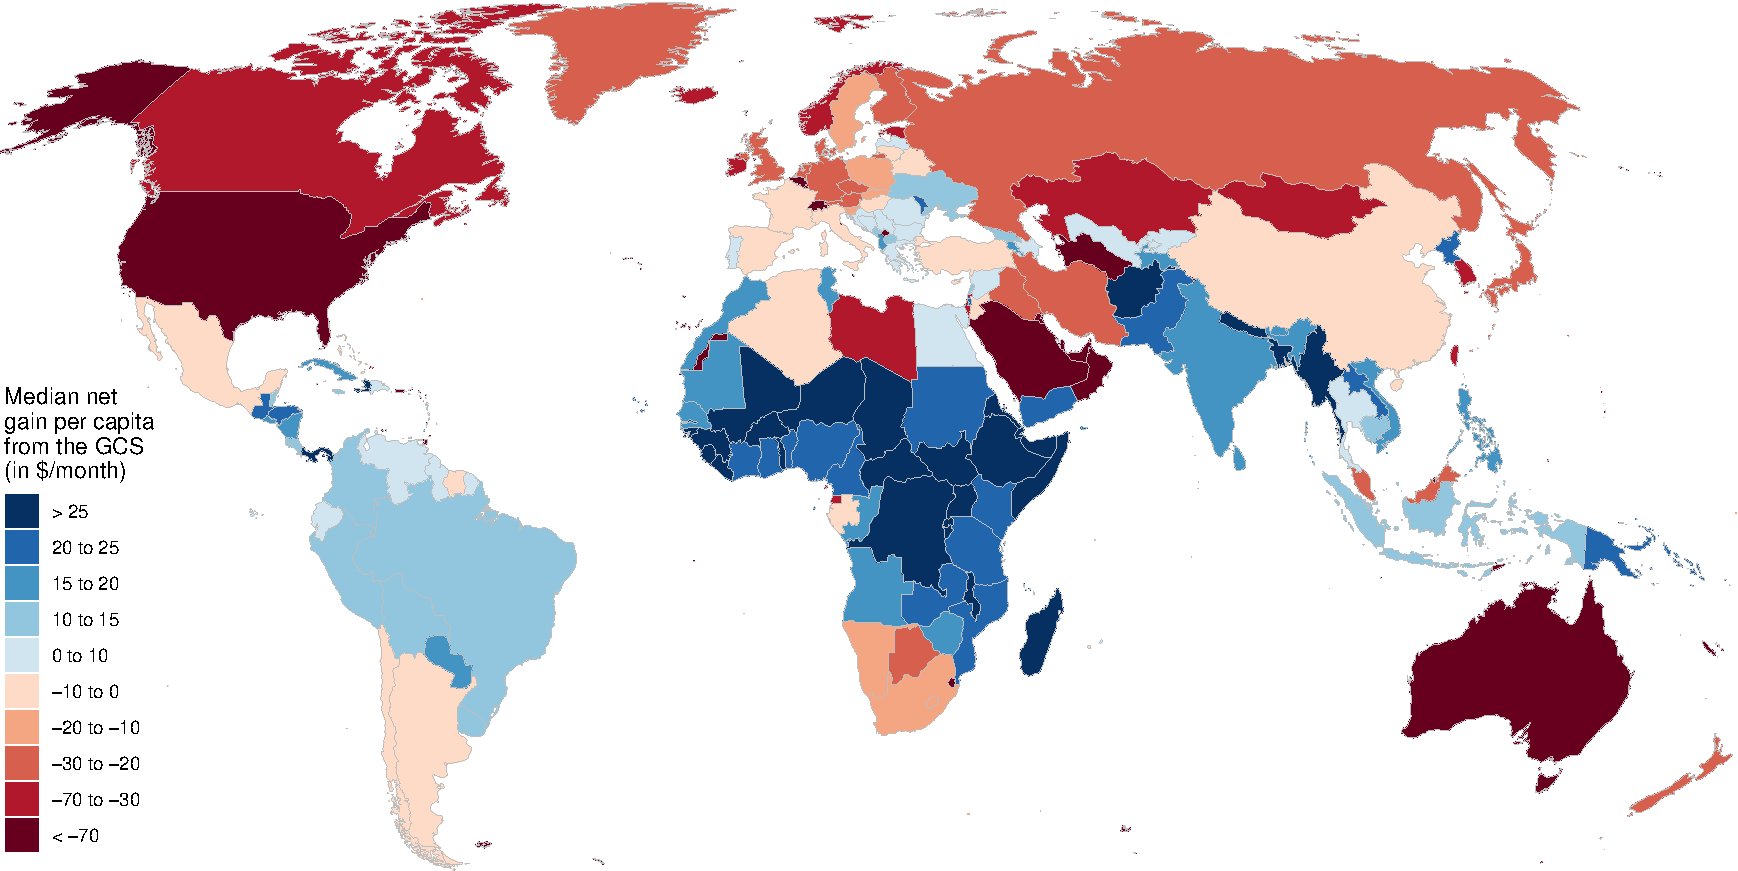
\includegraphics[width=\textwidth]{../figures/maps/median_gain_2015.pdf}} 
\end{figure}

% \begin{table}[h]\label{tab:gain_gcs}
%     \caption{Net gains from the Global Climate Scheme.} 
%     \makebox[\textwidth][c]{
        % \resizebox*{!}{.7\textheight}{
\clearpage
\begin{multicols}{2}
    \setbox\ltmcbox\vbox{
    \makeatletter\col@number\@ne
        
\begin{longtable}[t]{lrr}
\caption{\label{tab:gain_gcs.tex}Estimated net gain from the GCS in 2030 and carbon footprint by country.}\\
\toprule
  & \makecell{Mean\\net gain\\from\\the GCS\\(\$/month)} & \makecell{CO$_\text{2}$\\footprint\\per adult\\in 2019\\(tCO$_\text{2}$/y)}\\
\midrule
Saudi Arabia & -93 & 24.0\\
United States & -77 & 21.0\\
Australia & -60 & 17.6\\
Canada & -56 & 16.7\\
South Korea & -50 & 15.6\\
Germany & -30 & 11.7\\
Russia & -29 & 11.5\\
Japan & -28 & 11.3\\
Malaysia & -21 & 10.0\\
Iran & -19 & 9.5\\
Poland & -19 & 9.5\\
United Kingdom & -18 & 9.4\\
China & -14 & 8.6\\
Italy & -13 & 8.4\\
South Africa & -11 & 8.0\\
France & -10 & 7.8\\
Iraq* & -8 & 7.4\\
Spain & -6 & 7.0\\
Turkey & -2 & 6.2\\
Algeria* & -1 & 6.0\\
Mexico & 2 & 5.6\\
Ukraine & 2 & 5.6\\
Uzbekistan* & 4 & 5.1\\
Argentina & 5 & 4.9\\
Thailand & 6 & 4.6\\
Egypt & 12 & 3.6\\
Indonesia & 13 & 3.3\\
Colombia & 15 & 3.0\\
Brazil & 15 & 2.9\\
Vietnam & 15 & 2.9\\
Peru & 16 & 2.8\\
Morocco & 16 & 2.7\\
North Korea* & 17 & 2.5\\
India & 18 & 2.4\\
Philippines & 18 & 2.3\\
Pakistan & 22 & 1.6\\
Bangladesh & 24 & 1.1\\
Nigeria & 25 & 1.0\\
Kenya & 25 & 0.9\\
Myanmar* & 26 & 0.9\\
Sudan* & 26 & 0.9\\
Tanzania & 27 & 0.5\\
Afghanistan* & 27 & 0.5\\
Uganda & 28 & 0.4\\
Ethiopia & 28 & 0.3\\
Venezuela & 29 & 0.3\\
DRC* & 30 & 0.1\\
\bottomrule
\end{longtable}
    \unskip
    \unpenalty
    \unpenalty}
    \unvbox\ltmcbox
\end{multicols}
        % }
%     }
    {\footnotesize \textit{Note}: %Emission data is from \cite{peters_synthesis_2012}. 
    Asterisks denote countries where footprint is missing and territorial emissions is used instead. %Estimation of net gains is described in the text. 
    Values differ from Figure \ref{fig:median_gain_2015} as this table present estimates of \textit{mean} net gain per adult in \textit{2030}, not at the present. Only the countries with more than 20 million adults (covering 87\% of the global total) are shown. 
    }
% \end{table}

% \clearpage
% \section{Sources}\label{app:sources}



\clearpage
\section{Attrition analysis}\label{app:attrition}

\begin{table}[h]\label{tab:attrition_US1}
    \caption{Attrition analysis for the US1 survey.} 
    \makebox[\textwidth][c]{
\resizebox*{!}{.73\textheight}{ % 73 is the max when there is a title
        \begin{tabular}{@{\extracolsep{5pt}}lccccc} 
\\[-1.8ex]\hline 
\hline \\[-1.8ex] 
\\[-1.8ex] & \makecell{Dropped out} & \makecell{Dropped out\\after\\socio-eco} & \makecell{Failed\\attention test} & \makecell{Duration\\(in min)} & \makecell{Duration\\below\\4 min} \\ 
\\[-1.8ex] & (1) & (2) & (3) & (4) & (5)\\ 
\hline \\[-1.8ex] 
Mean & 0.091 & 0.074 & 0.073 & 21.595 & 0.018  \\ \hline \\[-1.8ex]
 Income quartile: 2 & $-$0.006 & $-$0.006 & $-$0.015 & $-$0.896 & $-$0.008 \\ 
  & (0.012) & (0.012) & (0.012) & (3.255) & (0.006) \\ 
  Income quartile: 3 & 0.0004 & 0.0004 & $-$0.023$^{**}$ & 0.424 & $-$0.002 \\ 
  & (0.014) & (0.014) & (0.011) & (2.872) & (0.007) \\ 
  Income quartile: 4 & $-$0.003 & $-$0.003 & $-$0.003 & $-$3.557 & 0.004 \\ 
  & (0.016) & (0.016) & (0.014) & (3.326) & (0.010) \\ 
  Diploma: Post secondary & $-$0.001 & $-$0.001 & 0.002 & 1.765 & 0.004 \\ 
  & (0.011) & (0.011) & (0.009) & (2.759) & (0.006) \\ 
  Age: 25-34 & $-$0.037$^{**}$ & $-$0.037$^{**}$ & 0.017 & $-$0.980 & $-$0.031$^{**}$ \\ 
  & (0.017) & (0.017) & (0.019) & (2.712) & (0.014) \\ 
  Age: 35-49 & $-$0.019 & $-$0.019 & $-$0.003 & 3.429 & $-$0.032$^{**}$ \\ 
  & (0.016) & (0.016) & (0.017) & (3.147) & (0.014) \\ 
  Age: 50-64 & $-$0.012 & $-$0.012 & $-$0.041$^{***}$ & 4.482 & $-$0.043$^{***}$ \\ 
  & (0.016) & (0.016) & (0.016) & (2.746) & (0.013) \\ 
  Age: 65+ & 0.068$^{***}$ & 0.068$^{***}$ & $-$0.047$^{***}$ & 7.702$^{*}$ & $-$0.051$^{***}$ \\ 
  & (0.020) & (0.020) & (0.016) & (4.623) & (0.013) \\ 
  Race: Hispanic & 0.004 & 0.004 & 0.004 & $-$5.499 & $-$0.009 \\ 
  & (0.017) & (0.017) & (0.018) & (3.541) & (0.010) \\ 
  Race: Other & $-$0.030 & $-$0.030 & 0.136$^{**}$ & $-$10.741$^{***}$ & 0.041 \\ 
  & (0.034) & (0.034) & (0.056) & (3.117) & (0.039) \\ 
  Race: White only & $-$0.037$^{***}$ & $-$0.037$^{***}$ & $-$0.011 & $-$7.882$^{**}$ & $-$0.005 \\ 
  & (0.013) & (0.013) & (0.014) & (3.131) & (0.009) \\ 
  Gender: Man & $-$0.051$^{***}$ & $-$0.051$^{***}$ & 0.022$^{**}$ & 0.314 & 0.003 \\ 
  & (0.009) & (0.009) & (0.009) & (2.580) & (0.005) \\ 
  Region: Northeast & $-$0.003 & $-$0.003 & 0.002 & $-$5.448 & $-$0.005 \\ 
  & (0.014) & (0.014) & (0.013) & (5.347) & (0.008) \\ 
  Region: South & $-$0.010 & $-$0.010 & 0.007 & $-$0.929 & $-$0.005 \\ 
  & (0.012) & (0.012) & (0.012) & (5.031) & (0.007) \\ 
  Region: West & 0.003 & 0.003 & $-$0.024$^{*}$ & $-$5.211 & $-$0.001 \\ 
  & (0.015) & (0.015) & (0.013) & (5.030) & (0.009) \\ 
  urbanTRUE & $-$0.004 & $-$0.004 & 0.011 & 5.009$^{**}$ & $-$0.006 \\ 
  & (0.011) & (0.011) & (0.010) & (2.451) & (0.007) \\ 
 \hline \\[-1.8ex] 

Observations & 4,226 & 4,226 & 2,817 & 2,661 & 2,661 \\ 
R$^{2}$ & 0.020 & 0.020 & 0.028 & 0.005 & 0.017 \\ 
\hline 
\hline \\[-1.8ex] 
\end{tabular} 
        }
    }
    {\footnotesize %\textit{Note}: 
    }
\end{table}

% \begin{table}[h]\label{tab:attrition_US2}
%     \caption{Attrition analysis for the US2 survey.} 
%     \makebox[\textwidth][c]{
% \resizebox*{!}{.73\textheight}{ % 73 is the max when there is a title
%         
\begin{tabular}{@{\extracolsep{5pt}}lccccc} 
\\[-1.8ex]\hline 
\hline \\[-1.8ex] 
\\[-1.8ex] & \makecell{Dropped out} & \makecell{Dropped out\\after\\socio-eco} & \makecell{Failed\\attention test} & \makecell{Duration\\(in min)} & \makecell{Duration\\below\\4 min} \\ 
\\[-1.8ex] & (1) & (2) & (3) & (4) & (5)\\ 
\hline \\[-1.8ex] 
Mean & 0.105 & 0.08 & 0.112 & 21.78 & 0.041  \\ \hline \\[-1.8ex]
 Income quartile: 3 & 0.007 & 0.007 & $-$0.053$^{***}$ & 1.441 & $-$0.043$^{***}$ \\ 
  & (0.022) & (0.022) & (0.020) & (3.244) & (0.015) \\ 
  Income quartile: 4 & 0.020 & 0.020 & $-$0.011 & 45.106 & $-$0.033 \\ 
  & (0.030) & (0.030) & (0.034) & (46.289) & (0.025) \\ 
  Diploma: Post secondary & $-$0.002 & $-$0.002 & $-$0.003 & 1.041 & $-$0.079$^{***}$ \\ 
  & (0.043) & (0.043) & (0.061) & (10.058) & (0.019) \\ 
  Age: 25-34 & $-$0.043$^{**}$ & $-$0.043$^{**}$ & $-$0.043$^{**}$ & 9.394 & 0.026 \\ 
  & (0.021) & (0.021) & (0.020) & (9.764) & (0.016) \\ 
  Age: 35-49 & 0.053$^{*}$ & 0.053$^{*}$ & $-$0.045 & $-$7.393 & 0.017 \\ 
  & (0.030) & (0.030) & (0.042) & (6.961) & (0.033) \\ 
  Age: 50-64 & 0.052$^{**}$ & 0.052$^{**}$ & $-$0.042 & 17.468 & 0.006 \\ 
  & (0.026) & (0.026) & (0.039) & (16.385) & (0.029) \\ 
  Age: 65+ & 0.066$^{**}$ & 0.066$^{**}$ & $-$0.071$^{*}$ & $-$7.421 & $-$0.042$^{*}$ \\ 
  & (0.029) & (0.029) & (0.040) & (9.109) & (0.025) \\ 
  Race: Black & 0.057$^{*}$ & 0.057$^{*}$ & $-$0.107$^{***}$ & $-$1.734 & $-$0.052$^{**}$ \\ 
  & (0.030) & (0.030) & (0.037) & (9.343) & (0.025) \\ 
  Race: Hispanic & 0.100$^{***}$ & 0.100$^{***}$ & $-$0.011 & 20.168 & $-$0.016 \\ 
  & (0.021) & (0.021) & (0.033) & (14.147) & (0.023) \\ 
  Gender: Man & 0.100$^{*}$ & 0.100$^{*}$ & 0.009 & $-$2.843 & 0.071 \\ 
  & (0.056) & (0.056) & (0.069) & (15.202) & (0.070) \\ 
  Region: Northeast & $-$0.050$^{***}$ & $-$0.050$^{***}$ & 0.015 & 13.563 & 0.017 \\ 
  & (0.018) & (0.018) & (0.023) & (16.255) & (0.017) \\ 
  Region: South & $-$0.018 & $-$0.018 & 0.030 & $-$4.964 & 0.014 \\ 
  & (0.030) & (0.030) & (0.043) & (4.837) & (0.029) \\ 
  Region: West & 0.013 & 0.013 & $-$0.029 & 10.628 & 0.007 \\ 
  & (0.024) & (0.024) & (0.034) & (13.411) & (0.022) \\ 
  Urban & 0.006 & 0.006 & $-$0.023 & 0.452 & 0.010 \\ 
  & (0.029) & (0.029) & (0.038) & (5.076) & (0.027) \\ 
  urban & 0.050$^{**}$ & 0.050$^{**}$ & 0.007 & 8.278 & 0.001 \\ 
  & (0.019) & (0.019) & (0.026) & (6.513) & (0.018) \\ 
 \hline \\[-1.8ex] 

Observations & 946 & 946 & 777 & 706 & 706 \\ 
R$^{2}$ & 0.042 & 0.042 & 0.046 & 0.023 & 0.043 \\ 
\hline 
\hline \\[-1.8ex] 
\end{tabular} 
%         }
%     }
%     {\footnotesize %\textit{Note}: 
%     }
% \end{table}

% \begin{table}[h]\label{tab:attrition_EU}
%     \caption{Attrition analysis for the EU survey.} 
%     \makebox[\textwidth][c]{
% \resizebox*{!}{.73\textheight}{ % 73 is the max when there is a title
%         
\begin{tabular}{@{\extracolsep{5pt}}lccccc} 
\\[-1.8ex]\hline 
\hline \\[-1.8ex] 
\\[-1.8ex] & \makecell{Dropped out} & \makecell{Dropped out\\after\\socio-eco} & \makecell{Failed\\attention test} & \makecell{Duration\\(in min)} & \makecell{Duration\\below\\6 min} \\ 
\\[-1.8ex] & (1) & (2) & (3) & (4) & (5)\\ 
\hline \\[-1.8ex] 
Mean & 0.067 & 0.044 & 0.151 & 54.602 & 0.039  \\ \hline \\[-1.8ex]
 Country: ES & $-$0.055$^{***}$ & $-$0.050$^{***}$ & 0.006 & $-$35.375$^{*}$ & $-$0.006 \\ 
  & (0.011) & (0.011) & (0.011) & (18.649) & (0.010) \\ 
  Country: FR & $-$0.020 & $-$0.016 & 0.031$^{***}$ & $-$5.377 & $-$0.012 \\ 
  & (0.012) & (0.012) & (0.012) & (20.286) & (0.009) \\ 
  Country: UK & 0.039$^{***}$ & 0.043$^{***}$ & 0.027$^{**}$ & $-$19.224 & $-$0.006 \\ 
  & (0.014) & (0.014) & (0.011) & (17.882) & (0.009) \\ 
  Income quartile: 2 & 0.003 & 0.001 & $-$0.028$^{**}$ & 29.027 & $-$0.016 \\ 
  & (0.012) & (0.012) & (0.013) & (20.302) & (0.010) \\ 
  Income quartile: 3 & $-$0.001 & $-$0.002 & $-$0.059$^{***}$ & 0.678 & $-$0.023$^{**}$ \\ 
  & (0.013) & (0.013) & (0.011) & (12.284) & (0.010) \\ 
  Income quartile: 4 & $-$0.028$^{*}$ & $-$0.029$^{**}$ & $-$0.045$^{***}$ & 11.603 & $-$0.019$^{*}$ \\ 
  & (0.014) & (0.014) & (0.013) & (18.776) & (0.010) \\ 
  Diploma: Post secondary & $-$0.007 & $-$0.007 & $-$0.033$^{***}$ & 7.918 & $-$0.008 \\ 
  & (0.011) & (0.010) & (0.009) & (12.848) & (0.007) \\ 
  Age: 25-34 & 0.022$^{*}$ & 0.019 & 0.031$^{*}$ & 36.191$^{*}$ & $-$0.004 \\ 
  & (0.013) & (0.013) & (0.019) & (21.496) & (0.018) \\ 
  Age: 35-49 & 0.049$^{***}$ & 0.047$^{***}$ & $-$0.008 & 34.108$^{**}$ & $-$0.013 \\ 
  & (0.013) & (0.013) & (0.016) & (15.221) & (0.016) \\ 
  Age: 50-64 & 0.070$^{***}$ & 0.068$^{***}$ & $-$0.011 & 45.820$^{**}$ & $-$0.063$^{***}$ \\ 
  & (0.014) & (0.014) & (0.017) & (21.671) & (0.015) \\ 
  Age: 65+ & 0.137$^{***}$ & 0.135$^{***}$ & $-$0.013 & 29.582$^{**}$ & $-$0.062$^{***}$ \\ 
  & (0.016) & (0.016) & (0.017) & (13.099) & (0.015) \\ 
  Gender: Man & $-$0.034$^{***}$ & $-$0.034$^{***}$ & 0.012 & $-$25.172$^{*}$ & 0.010 \\ 
  & (0.009) & (0.009) & (0.009) & (14.587) & (0.007) \\ 
  Degree of urbanization: Towns and suburbs & 0.004 & 0.002 & $-$0.017$^{*}$ & $-$15.348 & 0.007 \\ 
  & (0.010) & (0.010) & (0.010) & (17.562) & (0.008) \\ 
  Degree of urbanization: Rural & $-$0.001 & $-$0.001 & $-$0.017 & $-$14.010 & 0.001 \\ 
  & (0.013) & (0.013) & (0.011) & (20.315) & (0.009) \\ 
 \hline \\[-1.8ex] 

Observations & 3,963 & 3,963 & 3,326 & 3,115 & 3,115 \\ 
R$^{2}$ & 0.038 & 0.038 & 0.024 & 0.004 & 0.024 \\ 
\hline 
\hline \\[-1.8ex] 
\end{tabular} 
%         }
%     }
%     {\footnotesize %\textit{Note}: 
%     }
% \end{table}